\documentclass[a4paper,12pt]{report}
\usepackage[T1]{fontenc}
\usepackage[utf8]{inputenc}
\usepackage[italian]{babel}
\usepackage{graphicx} % Per le immagini
\usepackage{enumitem} % Liste numerate
\usepackage{tabularx} % Per tabelle
\usepackage{booktabs} % Per tabelle
\usepackage{float} % Per bloccare le immagini
\usepackage{url}
\usepackage{longtable}
\usepackage{dirtree}
\usepackage{pgfgantt} % strumento per generare GANTT

\title{Relazione Tecnica di Progetto \\ \large Wiki Collaborativo per Appunti}
\author{Domenico Aloi}
\date{Anno Accademico 2025/26 - Ingegneria del Software}

\begin{document}

\maketitle

\tableofcontents % Genera l'indice

\chapter{Introduzione}

\noindent La richiesta consiste nel creare un sistema dove gli studenti possono caricare, modificare e
versionare appunti per i corsi. 
Principalmente si tratterà di un editor di testo (semplice markdown o text-area) dotato di cronologia
delle versioni (semplificata) e un'organizzazione per corso/argomento.

\section{As-Is}
L'attuale gestione e condivisione degli appunti tra gli studenti universitari avviene prevalentemente in modo frammentato e manuale. Gli appunti sono dispersi su diverse piattaforme (email, chat, cloud personali), rendendo difficile la reperibilità del materiale. Non avendo un sistema centralizzato è altamente probabile disperdere correzzioni o aggiornamenti importanti. In questo contesto la collaborazione risulta molto complicata e limitata all'iniziativa personale.

\section{To-Be}
Il sistema \textbf{Wiki Collaborativo per Appunti} si propone di a risolvere tali problematiche attraverso un sistema centralizzato di collaborazione tra gli studenti. Esso infatti permetterà di:

\begin{itemize}
    \item \textbf{Condividere il materiale:} Gli appunti sono condivisi in un unico sistema alla portata di tutti e a disposizione di tutti.
    \item \textbf{Collaborare:} Ogni utente, dopo la registrazione, può contribuire aggiugnendo nuovi appunti o modificando gli esistenti.
    \item \textbf{Controllare il materiale:} Ogni modifica agli appunti genera automaticamente una nuova versione. Questo consente agli utenti di navigare nella cronologia e, in caso di errori rilevati, ripristinare la vecchia versione di un appunto.
\end{itemize} 
\chapter{Requisiti}

\section{Requisiti Funzionali (RF)}

\begin{enumerate}[label=\textbf{RF\arabic*}, widest=RF10, leftmargin=*, align=left]
    \item \textbf{Registrazione utente}
        \begin{itemize}[nosep, leftmargin=0cm]
            \item L'utente può creare un account fornendo email e password.
            \item Non è richiesto un sistema di validazione dell'email.
        \end{itemize}

    \item \textbf{Login/Logout}
        \begin{itemize}[nosep, leftmargin=0cm]
            \item L'utente può accedere al sistema tramite credenziali e terminare la sessione (logout).
        \end{itemize}

    \item \textbf{Visualizzazione corsi}
        \begin{itemize}[nosep, leftmargin=0cm]
            \item Qualsiasi utente (autenticato o visitatore) può visualizzare l'elenco dei corsi disponibili.
        \end{itemize}

    \item \textbf{Visualizzazione argomenti di un corso}
        \begin{itemize}[nosep, leftmargin=0cm]
            \item Ogni corso presenta una lista di argomenti.
            \item L'utente può navigare agevolmente tra i corsi e i relativi argomenti.
        \end{itemize}

    \item \textbf{Visualizzazione degli appunti}
        \begin{itemize}[nosep, leftmargin=0cm]
            \item L'utente può visualizzare gli appunti associati a un argomento.
            \item Ogni appunto è leggibile; il contenuto è visualizzato in formato HTML renderizzato (da sorgente Markdown o testo semplice).
        \end{itemize}

    \item \textbf{Creazione appunti}
        \begin{itemize}[nosep, leftmargin=0cm]
            \item Gli utenti autenticati possono creare nuovi appunti.
            \item Inserimento obbligatorio del titolo.
            \item Ogni appunto fa riferimento ad un solo corso ed un solo argomento.
        \end{itemize}

    \item \textbf{Modifica appunti}
        \begin{itemize}[nosep, leftmargin=0cm]
            \item Gli utenti autenticati hanno il permesso di modificare gli appunti esistenti.
            \item Ogni operazione di modifica genera automaticamente una nuova versione dell'appunto.
        \end{itemize}

    \item \textbf{Cronologia delle versioni}
        \begin{itemize}[nosep, leftmargin=0cm]
            \item Visualizzazione dell'elenco delle versioni precedenti per ogni appunto (inclusi timestamp e autore).
            \item Possibilità di consultare una versione specifica del passato.
            \item Funzionalità di ripristino: una versione precedente può essere promossa a versione attuale.
        \end{itemize}

    \item \textbf{Ricerca}
        \begin{itemize}[nosep, leftmargin=0cm]
            \item Sistema di ricerca per individuare appunti tramite il titolo.
        \end{itemize}

    \item \textbf{Gestione corsi, argomenti e appunti}
        \begin{itemize}[nosep, leftmargin=0cm]
            \item Gli utenti con privilegi di amministratore possono creare, modificare o eliminare corsi, argomenti. 
            \item Gli appunti sono eliminabili solo dall'amministratore.
        \end{itemize}
\end{enumerate}

\section{Requisiti Non Funzionali (RNF)}

\begin{enumerate}[label=\textbf{RNF\arabic*}, widest=RNF8, leftmargin=*, align=left]
    \item \textbf{Architettura}
        \begin{itemize}[nosep, leftmargin=0cm]
            \item L'applicazione deve essere sviluppata seguendo il pattern architetturale Model–View–Presenter (MVP).
            \item Frontend e Backend devono essere completamente disaccoppiati e comunicare esclusivamente tramite API.
        \end{itemize}

    \item \textbf{Tecnologie}
        \begin{itemize}[nosep, leftmargin=0cm]
            \item Frontend: utilizzo di tecnologie standard (HTML5, CSS3, JavaScript). È consentito l'uso di Bootstrap o jQuery.
            \item Backend: sviluppo in PHP puro (senza l'ausilio di framework come Laravel o Symfony).
            \item Interfaccia API: implementazione di servizi RESTful per le operazioni CRUD.
            \item Divieto di Server-Side Rendering (SSR): il backend non deve generare codice HTML.
        \end{itemize}

    \item \textbf{Indipendenza Frontend/Backend}
        \begin{itemize}[nosep, leftmargin=0cm]
            \item Il frontend deve essere progettato per poter interagire con backend alternativi (es. Java, Go).
            \item Il backend deve poter servire client differenti, inclusi dispositivi mobile o applicazioni desktop.
        \end{itemize}

    \item \textbf{Sicurezza}
        \begin{itemize}[nosep, leftmargin=0cm]
            \item Tutte le API che comportano la modifica dei dati devono essere protette tramite token di autenticazione o gestione della sessione.
            \item Le password devono essere memorizzate nel database esclusivamente tramite algoritmi di hashing sicuri.
            \item \textbf{Nota sulla produzione:} Sebbene il prototipo operi in locale su HTTP, per la messa in produzione è previsto l'uso del protocollo HTTPS per garantire la cifratura dei dati e la sicurezza delle sessioni
        \end{itemize}

    \item \textbf{Usabilità}
        \begin{itemize}[nosep, leftmargin=0cm]
            \item L'interfaccia utente deve seguire un design semplice, pulito e minimalista.
            \item Il sistema deve essere \textit{responsive}, garantendo il supporto ai dispositivi mobili.
        \end{itemize}

    \item \textbf{Prestazioni}
        \begin{itemize}[nosep, leftmargin=0cm]
            \item Il tempo di risposta del sistema per le tutte operazioni in condizioni di carico standard deve essere inferiore ai 5 secondi.
        \end{itemize}

    \item \textbf{Documentazione}
        \begin{itemize}[nosep, leftmargin=0cm]
            \item Il repository GitHub del progetto deve includere: requisiti, diagrammi UML, guida all'installazione e manuale utente sintetico.
        \end{itemize}

    \item \textbf{Versionamento}
        \begin{itemize}[nosep, leftmargin=0cm]
            \item Corretto utilizzo di Git e GitHub: gestione dei branch, commit regolari e descrittivi.
        \end{itemize}
\end{enumerate}
 
\chapter{Glossario}
\newpage
\begin{table}[H]
    \small
    \centering
    \caption{Glossario dei termini principali del sistema Wiki Collaborativo}
    \label{tab:glossario}
    \begin{tabularx}{\textwidth}{@{}l X@{}}
        \toprule
        \textbf{Termine} & \textbf{Definizione} \\
        \midrule
        \textbf{Amministratore} & Utente con privilegi elevati incaricato della gestione strutturale di corsi e argomenti. \\
        & \textit{Sinonimi: Admin.} \\
        \midrule
        \textbf{Appunto} & L'unità informativa principale del sistema, contenente testo in formato Markdown o plain text renderizzato in HTML. \\
        \midrule
        \textbf{Argomento} & Sotto-categoria tematica di un corso a cui vengono associati uno o più appunti. \\
        \midrule
        \textbf{Corso} & Categoria tematica a cui vengono associati uno o più argomenti. \\
        \midrule
        \textbf{CRUD} & Acronimo di Create, Read, Update, Delete; rappresenta le quattro operazioni di base gestite dalle API REST del sistema. \\
        \midrule
        \textbf{Markdown} & Linguaggio di markup leggero utilizzato dagli studenti per la formattazione del testo degli appunti. \\
        \midrule
        \textbf{MVP} & Pattern architetturale (Model-View-Presenter) che separa la logica di business dalla visualizzazione, come richiesto dai requisiti di progetto. \\
        \midrule
        \textbf{REST API} & Interfaccia programmabile stateless che permette la comunicazione tramite protocollo HTTP tra il frontend (JS) e il backend (PHP). \\
        \midrule
        \textbf{Studente} & Utente registrato che ha effettuato l'accesso e possiede i permessi per creare o modificare appunti e visualizzare la cronologia. \\
        & \textit{Sinonimi: Autore, Stud., StudAuth.} \\
        \midrule
        \textbf{Versione} & Stato storico di un appunto salvato in seguito a una modifica o a un ripristino. Consente di navigare nella cronologia dei contenuti e di recuperare checkpoint precedenti. \\
        & \textit{Sinonimi: Storico, Cronologia, Checkpoint.} \\
        \midrule
        \textbf{Visitatore} & Utente non registrato che non ha effettuato l'accesso. Può solo visualizzare e cercare gli appunti senza poterli creare o modificare. \\
        & \textit{Sinonimi: Visit.} \\
        \bottomrule
    \end{tabularx}
\end{table} 
\chapter{Diagrammi dei casi d'uso}
\noindent Il rettangolo nel diagramma rappresenta sempre il sistema \textbf{Wiki Collaborativo per Appunti}, ovvero il \textbf{soggetto}. La modellazione dei casi d’uso è stata articolata in base ai ruoli interpretati dagli attori esterni, al fine di evidenziare il \textbf{disaccoppiamento} tra le funzionalità pubbliche e quelle riservate:

\begin{itemize}[]
    \item \textbf{Visitatore}: rappresenta l'utente non autenticato che consulta il materiale.
    \item \textbf{Studente}: utente autenticato con permessi di contribuzione.
    \item \textbf{Amministratore}: ruolo preposto alla gestione strutturale di corsi e argomenti.
\end{itemize}

\noindent Sotto il profilo della modellazione, sia il ruolo \textbf{Studente} che il ruolo \textbf{Amministratore} sono rappresentati come generalizzazioni del \textbf{Visitatore}. Questa astrazione permette di indicare che entrambi i ruoli autenticati ereditano implicitamente tutti i casi d’uso di consultazione e ricerca (\textbf{RF3, RF4, RF9}) senza appesantire graficamente il diagramma con linee ridondanti.
Tuttavia, si evidenziano due importanti eccezioni alla gerarchia dei permessi:


\begin{itemize}[]
    \item \textbf{Esclusione del caso d'uso Registrazione (RF1)}: Una volta autenticati, né lo \textbf{Studente} né l'\textbf{Amministratore} possono accedere alla funzione di registrazione, in quanto lo stato di utente loggato è logicamente incompatibile con la creazione di un nuovo account.
    \item \textbf{Vincoli sulla creazione degli account}: In linea con i requisiti di sicurezza, la funzione di registrazione pubblica è limitata esclusivamente al ruolo \textbf{Studente}. Il ruolo \textbf{Amministratore} non può essere ottenuto tramite registrazione autonoma (per prevenire scalate di privilegi non autorizzate), ma viene gestito esclusivamente a livello di persistenza tramite l'inserimento manuale o script di inizializzazione nel database.
\end{itemize}

\noindent Ho diviso i diagrammi per attore per rendere più chiara la separazione delle responsabilità e dei permessi di accesso, facilitando la tracciabilità tra i requisiti funzionali e le interazioni modellate .

\section{Dettagli del Caso d'Uso UC1}

\begin{figure}[H] % h=here, t=top, b=bottom, p=page [8, 9]
    \centering
    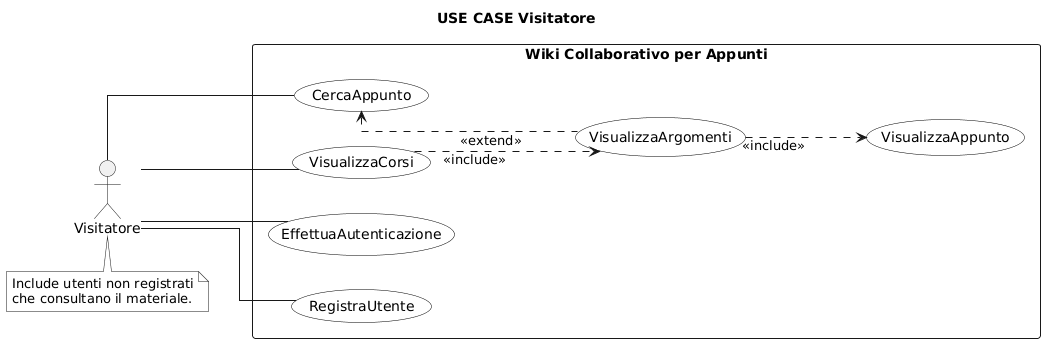
\includegraphics[width=1\textwidth]{UseCase/visitatore.png} % [10, 11]
    \caption{UC1 - Diagramma dei casi d'uso per l'attore Visitatore}
    \label{fig:uc_visitatore} % [12, 13]
\end{figure}

\begin{table}[H]
    \small
    \caption{Specifica del caso d'uso per RF1: RegistraUtente}
    \begin{tabularx}{\textwidth}{@{}l X@{}}
        \toprule
        \textbf{ID} & 1 \\
        \midrule
        \textbf{Nome} & \textbf{RegistraUtente} \\
        \midrule
        \textbf{Descrizione} & Permette a un nuovo utente di creare un account fornendo email e password. \\
        \midrule
        \textbf{Attori} & Visitatore. \\
        \midrule
        \textbf{Precondizioni} & L'utente non è registrato. \\
        \midrule
        \textbf{Flusso Principale} & 
        1. L'utente seleziona la funzione di registrazione. \newline
        2. L'utente inserisce email e password. \newline
        2. Il sistema valida il formato dei dati (es. email valida). \newline
        4. Il sistema esegue l'hashing della password per sicurezza. \newline
        5. Il sistema memorizza i dati nel database. \\
        \midrule
        \textbf{Postcondizioni} & Un nuovo account è stato creato con successo. \\
        \midrule
        \textbf{Flussi Alternativi} & \textbf{A1. Email già presente:} Il sistema informa l'utente che l'email è già registrata e interrompe la procedura. \\
        \bottomrule
    \end{tabularx}
\end{table}

\begin{table}[H]
    \small
    \caption{Specifica del caso d'uso per RF2: EffettuaAutenticazione}
    \begin{tabularx}{\textwidth}{@{}l X@{}}
        \toprule
        \textbf{ID} & 2 \\
        \midrule
        \textbf{Nome} & \textbf{EffettuaAutenticazione} \\
        \midrule
        \textbf{Descrizione} & Consente all'utente di accedere al sistema tramite le proprie credenziali. \\
        \midrule
        \textbf{Attori} & Visitatore. \\
        \midrule
        \textbf{Precondizioni} & L'utente deve possedere un account registrato. \\
        \midrule
        \textbf{Flusso Principale} & 
        1. L'utente accede alla funzione di login. \newline
        2. L'utente inserisce email e password. \newline
        3. Il sistema confronta le credenziali con quelle nel database. \newline
        4. Il sistema avvia una sessione autenticata. \\
        \midrule
        \textbf{Postcondizioni} & L'utente è autenticato e in base al suo ruolo può accedere alle funzioni di creazione/modifica. \\
        \midrule
        \textbf{Flussi Alternativi} & \textbf{A1. Credenziali errate:} Il sistema nega l'accesso e mostra un messaggio di errore. \\
        \bottomrule
    \end{tabularx}
\end{table}

\begin{table}[H]
    \small
    \caption{Specifica del caso d'uso per RF3: VisualizzaCorsi}
    \begin{tabularx}{\textwidth}{@{}l X@{}}
        \toprule
        \textbf{ID} & 3 \\
        \midrule
        \textbf{Nome} & \textbf{VisualizzaCorsi} \\
        \midrule
        \textbf{Descrizione} & Permette di consultare l'elenco completo dei corsi disponibili nel Wiki. \\
        \midrule
        \textbf{Attori} & Visitatore. \\
        \midrule
        \textbf{Precondizioni} & Il sistema è accessibile. \\
        \midrule
        \textbf{Flusso Principale} & 
        1. L'utente accede alla pagina principale. \newline
        2. In automatico il sistema recupera i nomi dei corsi dal database. \newline
        3. Il sistema mostra l'elenco dei corsi all'utente. \\
        \midrule
        \textbf{Postcondizioni} & L'utente visualizza l'elenco dei corsi. \\
        \bottomrule
    \end{tabularx}
\end{table}

\begin{table}[H]
    \small
    \caption{Specifica del caso d'uso per RF4: VisualizzaArgomenti}
    \begin{tabularx}{\textwidth}{@{}l X@{}}
        \toprule
        \textbf{ID} & 4 \\
        \midrule
        \textbf{Nome} & \textbf{VisualizzaArgomenti} \\
        \midrule
        \textbf{Descrizione} & Permette di navigare tra gli argomenti associati a un corso specifico. \\
        \midrule
        \textbf{Attori} & Visitatore. \\
        \midrule
        \textbf{Precondizioni} & L'utente ha selezionato un corso (3). \\
        \midrule
        \textbf{Flusso Principale} & 
        1. L'utente seleziona un corso. \newline
        2. Il sistema recupera gli argomenti legati a quel corso. \newline
        3. Il sistema mostra la lista degli argomenti di quel corso. \\
        \midrule
        \textbf{Postcondizioni} & L'utente visualizza gli appunti collegati a quell'argomento. \\
        \bottomrule
    \end{tabularx}
\end{table}

\begin{table}[H]
    \small
    \caption{Specifica del caso d'uso per RF5: VisualizzaAppunto}
    \begin{tabularx}{\textwidth}{@{}l X@{}}
        \toprule
        \textbf{ID} & 5 \\
        \midrule
        \textbf{Nome} & \textbf{VisualizzaAppunto} \\
        \midrule
        \textbf{Descrizione} & Mostra il contenuto di un appunto in formato HTML renderizzato. \\
        \midrule
        \textbf{Attori} & Visitatore. \\
        \midrule
        \textbf{Precondizioni} & L'utente ha selezionato un corso e un argomento (4). \\
        \midrule
        \textbf{Flusso Principale} & 
        1. L'utente seleziona un appunto. \newline
        2. Il sistema recupera il testo (Markdown/Plain text) dal database. \newline
        3. Il sistema converte il testo in HTML e lo visualizza. \\
        \midrule
        \textbf{Postcondizioni} & L'utente visualizza l'appunto renderizzato. \\
        \bottomrule
    \end{tabularx}
\end{table}

\begin{table}[H]
    \small
    \caption{Specifica del caso d'uso per RF9: CercaAppunto}
    \begin{tabularx}{\textwidth}{@{}l X@{}}
        \toprule
        \textbf{ID} & 9 \\
        \midrule
        \textbf{Nome} & \textbf{CercaAppunto} \\
        \midrule
        \textbf{Descrizione} & Permette la ricerca di appunti tramite titolo, contenuto o corso. \\
        \midrule
        \textbf{Attori} & Visitatore. \\
        \midrule
        \textbf{Precondizioni} & Il sistema è operativo. \\
        \midrule
        \textbf{Flusso Principale} & 
        1. L'utente inserisce una stringa nella funzione di ricerca. \newline
        2. Il sistema interroga il database cercando corrispondenze nei titoli. \newline
        3. Il sistema mostra i risultati filtrati. \\
        \midrule
        \textbf{Postcondizioni} & L'utente seleziona un appunto dai risultati (prosegue con 5). \\
        \bottomrule
    \end{tabularx}
\end{table}


\section{Dettagli del Caso d'Uso UC2}

\begin{figure}[H] % h=here, t=top, b=bottom, p=page [8, 9]
    \centering
    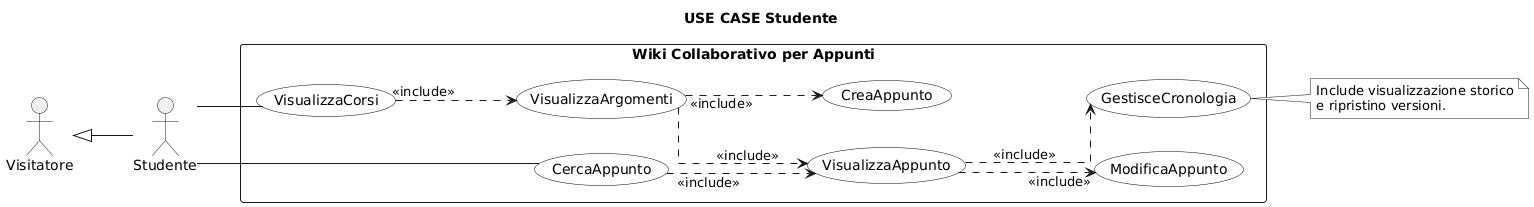
\includegraphics[width=1\textwidth]{UseCase/stud.png} % [10, 11]
    \caption{UC2 - Diagramma dei casi d'uso per l'attore Studente}
    \label{fig:uc_studente} % [12, 13]
\end{figure}

\begin{table}[H]
    \small
    \caption{Specifica del caso d'uso per RF6: CreaAppunto}
    \label{tab:spec_uc6}
    \begin{tabularx}{\textwidth}{@{}l X@{}}
        \toprule
        \textbf{ID} & 6 \\
        \midrule
        \textbf{Nome} & \textbf{CreaAppunto} \\
        \midrule
        \textbf{Descrizione} & Permette a un utente autenticato di inserire un nuovo appunto nel sistema associandolo a un corso e a un argomento specifico. \\
        \midrule
        \textbf{Attori} & Studente. \\
        \midrule
        \textbf{Precondizioni} & L'utente ha effettuato il login (2) e si trova nella sezione di visualizzazione degli appunti per argomento (4). \\
        \midrule
        \textbf{Flusso Principale} & 
        1. L'utente seleziona la funzione "Crea Nuovo Appunto". \newline
        2. L'utente inserisce il titolo dell'appunto. \newline
        3. L'utente inserisce il contenuto testuale (Markdown o Plain Text). \newline
        4. L'utente conferma il salvataggio. \newline
        5. Il sistema valida i dati, memorizza l'appunto e associa l'ID dell'autore. \\
        \midrule
        \textbf{Postcondizioni} & Il nuovo appunto è persistente nel database. \\
        \midrule
        \textbf{Flussi Alternativi} & \textbf{A1. Dati mancanti:} Se il titolo è vuoto, il sistema non procede al salvataggio. \\
        \bottomrule
    \end{tabularx}
\end{table}

\begin{table}[H]
    \small
    \caption{Specifica del caso d'uso per RF7: ModificaAppunto}
    \label{tab:spec_uc7}
    \begin{tabularx}{\textwidth}{@{}l X@{}}
        \toprule
        \textbf{ID} & 7 \\
        \midrule
        \textbf{Nome} & \textbf{ModificaAppunto} \\
        \midrule
        \textbf{Descrizione} & Consente a un utente autenticato di modificare il testo di un appunto esistente. Ogni modifica genera automaticamente una nuova versione nella cronologia. \\
        \midrule
        \textbf{Attori} & Studente. \\
        \midrule
        \textbf{Precondizioni} & L'utente è autenticato e ha visualizzato l'appunto che intende modificare (5). \\
        \midrule
        \textbf{Flusso Principale} & 
        1. L'utente esegue apporta al testo le modifiche desiderate. \newline
        2. L'utente seleziona la funzione "Salva Nuova Versione" . \newline
        3. Il sistema salva le modifiche e genera automaticamente una nuova voce nella cronologia con timestamp e ID autore. \\
        \midrule
        \textbf{Postcondizioni} & La versione corrente dell'appunto è aggiornata; la versione precedente è conservata nello storico (RF8). \\
        \midrule
        \textbf{Flussi Alternativi} & \textbf{A1. Annullamento:} L'utente esce dall'editor senza salvare; il sistema non apporta modifiche e non crea nuove versioni. \\
        \bottomrule
    \end{tabularx}
\end{table}

\begin{table}[H]
    \small
    \caption{Specifica del caso d'uso per RF8: GestisceCronologia}
    \label{tab:spec_uc8}
    \begin{tabularx}{\textwidth}{@{}l X@{}}
        \toprule
        \textbf{ID} & 8 \\
        \midrule
        \textbf{Nome} & \textbf{GestisceCronologia} \\
        \midrule
        \textbf{Descrizione} & Permette di visualizzare l'elenco delle versioni precedenti di un appunto e di effettuarne il ripristino. \\
        \midrule
        \textbf{Attori} & Studente. \\
        \midrule
        \textbf{Precondizioni} & L'appunto selezionato ha subito almeno una modifica (esiste uno storico versioni), l'utente si trova nella visualizzazione dell'appunto (5). \\
        \midrule
        \textbf{Flusso Principale} & 
        1. L'utente seleziona la voce "Vedi Cronologia". \newline
        2. Il sistema mostra l'elenco delle versioni (timestamp e autore della modifica). \newline
        3. L'utente seleziona una versione precedente per visualizzarla. \newline
        4. L'utente richiede il ripristino della versione selezionata. \newline
        5. Il sistema sovrascrive la versione attuale con quella scelta, rendendola la più recente. \\
        \midrule
        \textbf{Postcondizioni} & L'appunto viene riportato allo stato della versione selezionata. \\
        \midrule
        \textbf{Flussi Alternativi} & \textbf{A1. Sola consultazione:} L'utente visualizza una versione passata ma non effettua il ripristino. \\
        \bottomrule
    \end{tabularx}
\end{table}

\newpage
\section{Dettagli del Caso d'Uso UC3}

\begin{figure}[H] % h=here, t=top, b=bottom, p=page [8, 9]
    \centering
    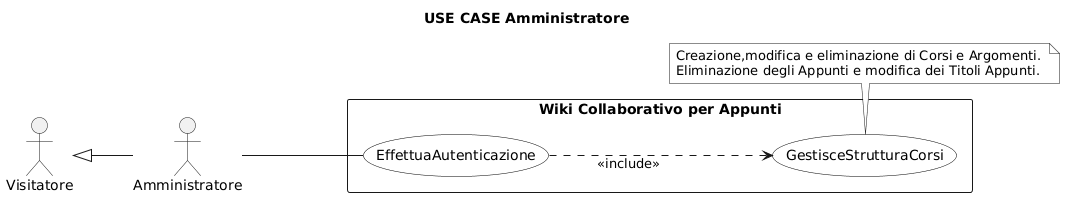
\includegraphics[width=1\textwidth]{UseCase/admin.png} % [10, 11]
    \caption{UC3 - Diagramma dei casi d'uso per l'attore Amministratore}
    \label{fig:uc_amministratore} % [12, 13]
\end{figure}

\begin{table}[H]
    \small
    \caption{Specifica del caso d'uso per RF2: EffettuaAutenticazione (Admin)}
    \label{tab:spec_uc2_admin}
    \begin{tabularx}{\textwidth}{@{}l X@{}}
        \toprule
        \textbf{ID} & 2 \\
        \midrule
        \textbf{Nome} & \textbf{EffettuaAutenticazione (Admin)} \\
        \midrule
        \textbf{Descrizione} & Consente all'Amministratore di accedere all'area gestionale del Wiki tramite credenziali riservate. \\
        \midrule
        \textbf{Attori} & Amministratore. \\
        \midrule
        \textbf{Precondizioni} & Il sistema è operativo e l'Amministratore possiede credenziali valide memorizzate tramite hashing. \\
        \midrule
        \textbf{Flusso Principale} & 
        1. L'Amministratore inserisce email e password nella pagina di login. \newline
        2. Il sistema invia i dati al backend tramite richiesta POST. \newline
        3. Il backend valida le credenziali confrontandole con i dati nel DB. \newline
        4. Il sistema avvia una sessione con privilegi elevati (Admin). \\
        \midrule
        \textbf{Postcondizioni} & L'Amministratore è autenticato e viene reindirizzato alla dashboard di gestione (11). \\
        \midrule
        \textbf{Flussi Alternativi} & \textbf{A1. Credenziali non valide:} Il sistema nega l'accesso e restituisce un errore JSON (status 401 Unauthorized). \\
        \bottomrule
    \end{tabularx}
\end{table}




\begin{table}[H]
    \small
    \caption{Specifica del caso d'uso per RF11: GestisceStrutturaCorsi}
    \label{tab:spec_uc11}
    \begin{tabularx}{\textwidth}{@{}l X@{}}
        \toprule
        \textbf{ID} & 11 \\
        \midrule
        \textbf{Nome} & \textbf{GestisceStrutturaCorsi} \\
        \midrule
        \textbf{Descrizione} & Permette all'Amministratore di creare, modificare o eliminare corsi e i relativi argomenti associati. \\
        \midrule
        \textbf{Attori} & Amministratore. \\
        \midrule
        \textbf{Precondizioni} & L'Amministratore ha effettuato con successo l'autenticazione (2). \\
        \midrule
        \textbf{Flusso Principale} & 
        1. L'Amministratore seleziona "Gestione Corsi" dalla dashboard. \newline
        2. Il sistema mostra l'elenco dei corsi esistenti recuperati dal DB. \newline
        3. L'Amministratore sceglie di inserire un nuovo corso o di modificarne uno esistente. \newline
        4. L'Amministratore inserisce, modifica e elimina corsi e argomenti. L'amministratore modifica i titoli degli appunti e elimina gli appunti. \newline
        5. Il sistema invia i dati al backend tramite REST API. \newline
        6. Il backend aggiorna le tabelle relazionali nel database. \\
        \midrule
        \textbf{Postcondizioni} & La nuova struttura dei corsi è salvata in modo persistente e visibile a tutti gli utenti (\textbf{RF3, RF4, RF5}). \\
        \bottomrule
    \end{tabularx}
\end{table}

\newpage
\section{Matrice di tracciabilità}
\begin{table}[htbp]
    \centering
    \caption{Matrice di tracciabilità}
    \begin{tabular}{lccc}
        \toprule
        Requisito Funzionale & UC1 (Visit.) & UC2 (Stud.) & UC3 (Admin) \\
        \midrule
        RF1 (Registrazione)  & X &   &   \\
        RF2 (Login/Logout)   &   & X & X \\
        RF3 (Lista corsi)    & X &   &   \\
        RF4 (Lista Argomenti)      & X &   &   \\
        RF5 (Visualizza appunto)& X &   &   \\
        RF6 (Crea appunto)   &   & X &   \\
        RF7 (Modifica appunto)       &   & X &   \\
        RF8 (Gestione Cronologia)     &   & X &   \\
        RF9 (Ricerca)        & X &   &   \\
        RF10 (Gestione Admin.)&   &   & X \\
        \bottomrule
    \end{tabular}
\end{table}
 
\chapter{Progettazione}

\noindent La fase di progettazione traduce i requisiti analizzati in una struttura tecnica definita, seguendo un approccio top-down. Inizialmente viene definita l'architettura macroscopica del sistema, per poi scendere nel dettaglio dei singoli componenti e delle loro interazioni dinamiche.

\section{Architettura Logica (Sottosistemi)}

\noindent In conformità con lo sforzo di progettazione ad alto livello richiesto, il sistema è stato suddiviso in \textbf{sottosistemi a compartimenti stagni}. Questa scelta garantisce l'indipendenza funzionale e facilita la manutenzione, permettendo a ogni modulo di evolvere senza impattare direttamente sugli altri.

\noindent L'architettura logica si articola in tre macro-moduli principali:

\begin{itemize}
    \item \textbf{Sottosistema di Presentazione (Frontend)}: Implementa il pattern \textbf{Model-View-Presenter (MVP)} in modalità \textit{Passive View}, assicurando che la logica di visualizzazione sia totalmente disaccoppiata dallo stato dei dati. La \textit{View} notifica gli eventi al \textit{Presenter}, il quale coordina l'aggiornamento del \textit{Model} locale.
    \item \textbf{Sottosistema di Logica di Business (Backend)}: Agisce come coordinatore centrale. Include i moduli \textit{Core} per l'instradamento delle richieste tramite \texttt{Router}, e i \textit{Table Data Gateway} per l'incapsulamento della logica \textit{SQL}. La sicurezza autoritativa è delegata a \textit{Protection Proxies}, mentre la generazione dinamica delle query è affidata al pattern \textit{Strategy}.
    \item \textbf{Sottosistema di Persistenza (Database)}: Modella la base di dati relazionale \texttt{wiki\_db}. L'interazione è mediata dall'astrazione \textit{PDO}. L'accesso a questo modulo è mediato interamente dal backend tramite il pattern \textit{Table Data Gateway}.
\end{itemize}

\noindent La Figura \ref{fig:package_diagram} illustra questa gerarchia attraverso un \textbf{Package Diagram} UML. Le frecce di dipendenza mostrano come il Frontend dipenda dal Backend per il recupero dei dati, e quest'ultimo dipenda dal Database per la persistenza, rispettando il principio del disaccoppiamento.

\begin{figure}[H]
    \centering
    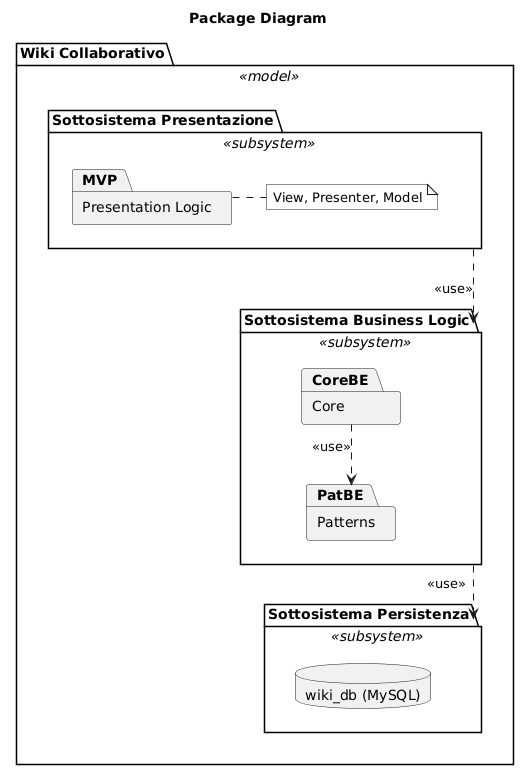
\includegraphics[width=0.7\textwidth]{AltriDiagrammi/PackDiag.png}
    \caption{Package Diagram}
    \label{fig:package_diagram}
\end{figure}

\section{Architettura Fisica (Deployment)}

\noindent L'architettura fisica del sistema è basata sulla tecnologia di containerizzazione \textbf{Docker}, che permette di isolare i sottosistemi in ambienti di esecuzione (nodi) indipendenti e riproducibili. La configurazione è definita tramite il file \texttt{docker-compose.yml}, che orchestra tre container distinti:

\begin{enumerate}
    \item \textbf{Container Frontend}: Utilizza l'immagine \texttt{httpd:alpine}. Espone il servizio sulla porta \textbf{8080} del PC-Host, servendo i file statici (HTML/CSS) e gli script JavaScript al browser dell’utente.
    \item \textbf{Container Backend}: Basato sull'immagine \texttt{php:8.2-apache}. Risponde sulla porta \textbf{8000} e gestisce la logica \texttt{PHP}. Include le estensioni \texttt{pdo\_mysql} necessarie per il dialogo con il database.
    \item \textbf{Container Database}: Utilizza \texttt{mysql:8.0} sulla porta interna \textbf{3306}. La persistenza è garantita da un volume dedicato (\texttt{db\_data}), assicurando che i dati sopravvivano al ciclo di vita del container.
\end{enumerate}

\noindent Tale configurazione soddisfa il requisito \textbf{RNF3 (Indipendenza)}, rendendo il backend e il frontend effettivamente intercambiabili con tecnologie alternative senza compromettere il funzionamento complessivo.

\begin{figure}[H]
    \centering
    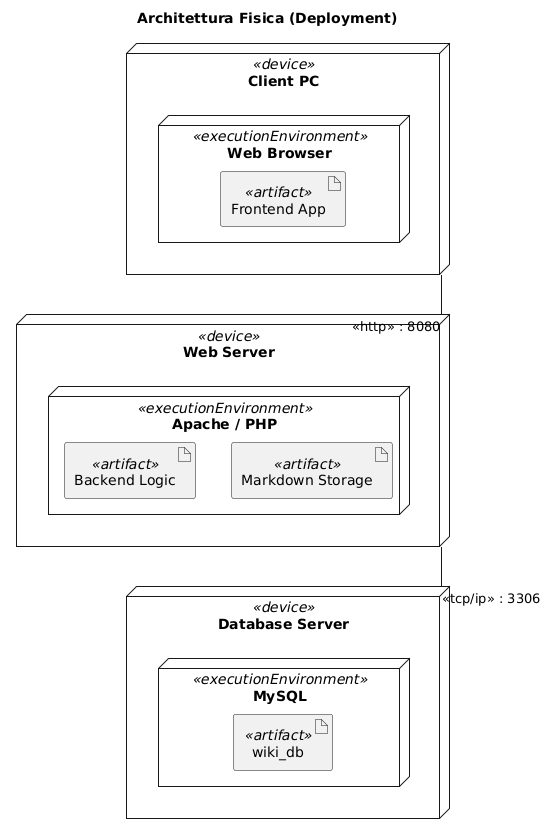
\includegraphics[width=0.6\textwidth]{AltriDiagrammi/deployment.png}
    \caption{Architettura Fisica (Deployment)}
    \label{fig:deployment}
\end{figure}

\section{Processo di Sviluppo e Gestione}

\subsection{Pianificazione delle Attività (Diagramma di GANTT)}

\noindent La pianificazione non segue una rigida successione di fasi, ma è articolata in task basati su obiettivi di progettazione. Ogni task comprende una sotto-fase di modellazione seguita dal refactoring del codice esistente per l'integrazione dei nuovi pattern.

\begin{center}
\begin{ganttchart}[
    expand chart=\textwidth,
    hgrid,
    vgrid,
    x unit=1.2cm,
    y unit title=0.7cm,
    y unit chart=0.8cm,
    title height=1,
    bar/.style={fill=blue!30, draw=blue!60},
    bar height=0.6,
    group/.style={fill=gray!20, draw=black},
    group right shift=0,
    group top shift=0.7,
    group height=.3,
    milestone/.style={fill=red, draw=red},
    milestone height=0.4
]{1}{8} 
    \gantttitle{Pianificazione (W1 - W4)}{8}\\
    \gantttitlelist{1,...,4}{2} \\
    
    \ganttbar{Struttura Iniziale (MVP/TDG)}{1}{1} \\
    \ganttbar{Core Functionality (FE/BE)}{2}{3} \\ 
    \ganttbar{Autenticazione (Strategy)}{4}{4} \\
    \ganttbar{Cronologia (Memento)}{5}{5} \\
    \ganttbar{Sicurezza e Privilegi (Proxy)}{6}{7} \\ 
    \ganttbar{Refactoring e Testing Finale}{8}{8} \\
    \ganttmilestone{Consegna Progetto}{8}
\end{ganttchart}
\captionof{Diagramma di Gantt: Sviluppo Sequenziale del Sistema}
\end{center}

\subsection{Metodologia di Sviluppo}
\noindent Lo sviluppo è stato condotto seguendo una metodologia \textbf{Agile/Scrum} adattata al singolo sviluppatore, caratterizzata da iterazioni brevi e rilasci incrementali di funzionalità (\textit{MVP}). A differenza dei modelli tradizionali, la progettazione architettonica non è stata completata interamente in modo preliminare, ma è evoluta attraverso cicli di \textbf{Refactor Mercilessly} . Questo ha permesso di scoprire la necessità di pattern specifici (come \textit{Memento} o \textit{Proxy}) solo a fronte di reali requisiti emersi durante la codifica, garantendo un design pulito e privo di sovra-progettazione (\textit{YAGNI}). La coerenza del codice è stata mantenuta tramite l'uso di \textbf{Git} per il controllo di versione e \textbf{Docker} per garantire l'uniformità dell'ambiente di esecuzione.

\subsection{Approccio allo Sviluppo}

\noindent Il sistema è stato suddiviso in moduli logici (``tronconi''), i quali rispecchiano la strategia di \textbf{branching} adottata nel repository Git per isolare lo sviluppo delle singole funzionalità prima del merge nel ramo principale. Seguendo un approccio di \textbf{sviluppo incrementale}, ogni passaggio è stato preceduto da una fase di design specifica per garantire che l'implementazione non degradasse la qualità architetturale complessiva.

\begin{itemize}
    \item \textbf{Struttura Iniziale}: Definizione dei pilastri (\textbf{MVP} e \textbf{Table Data Gateway}) per la separazione $FE/BE$ e l'astrazione del DB.
    \item \textbf{Consultazione Appunti}: Stabilite le basi REST API e la gestione del File System.
    \item \textbf{Autenticazione}: Introduzione del pattern \textbf{Strategy} per gestire i criteri di filtraggio utenti e l'hash delle password.
    \item \textbf{Cronologia}: Implementazione del pattern \textbf{Memento} per il salvataggio atomico degli stati storici sul file system.
    \item \textbf{Privilegi e Sicurezza}: Integrazione del pattern \textbf{Protection Proxy} per centralizzare l'autorizzazione senza inquinare la logica dei Gateway.
    \item \textbf{Refactoring Finale}: Scomposizione del \textbf{God Object} \texttt{index.php} in una gerarchia di \texttt{Controller} e \texttt{Router}, ottimizzando la manutenibilità e la "salute" del codice sorgente, abbellimenti al FE, varie fix e aggiunta di qualche funzione extra(come l'anteprima live e il download in pdf).
\end{itemize}

\section{Diagrammi delle Classi}

\noindent I diagrammi delle classi descrivono i tipi di oggetti del sistema e le loro \textbf{relazioni statiche}. Essi formalizzano la struttura del software dettagliando attributi, operazioni e vincoli di ogni componente, comprese le classi che ne definiscono il \textbf{comportamento}.

\subsection{Diagramma delle Classi FE}

\noindent Il diagramma illustra l'architettura del client basata sul pattern \textbf{MVP (Model-View-Presenter)}, finalizzata alla separazione tra logica di presentazione e visualizzazione.

\begin{figure}[H]
    \centering
    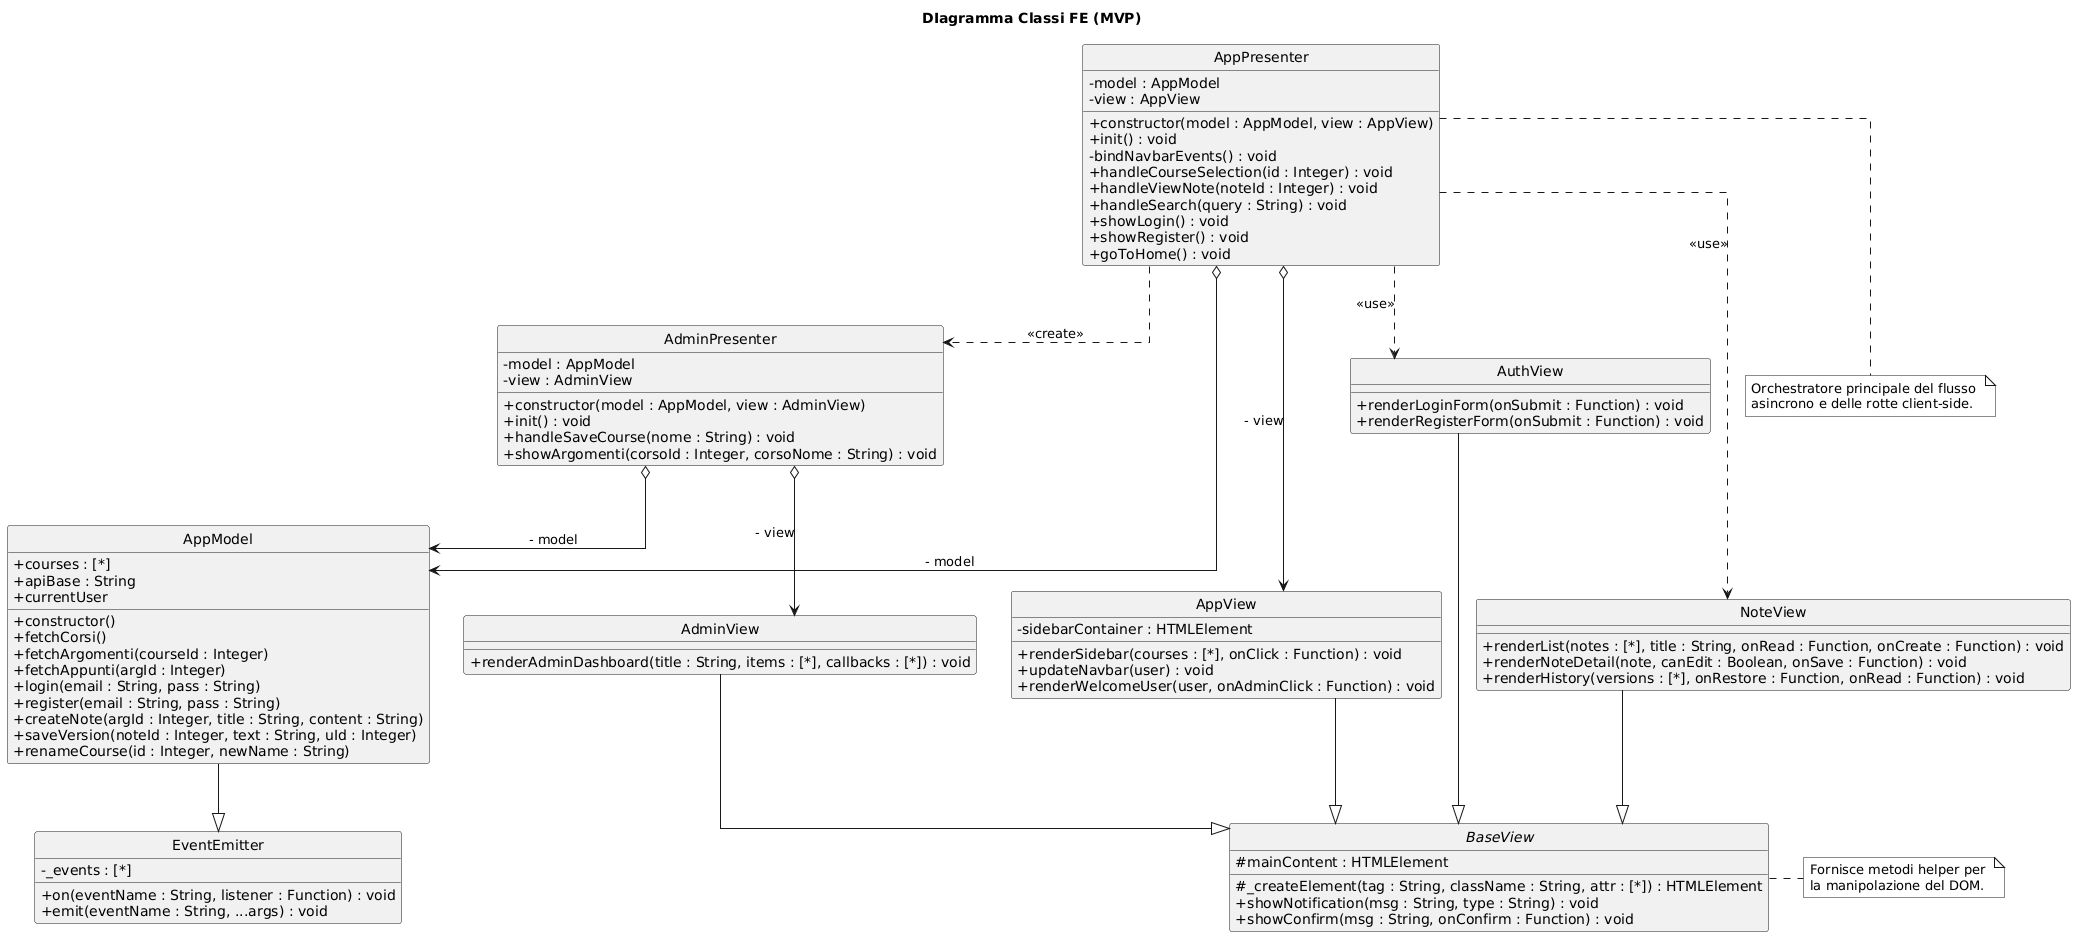
\includegraphics[width=1\textwidth]{DiagrammiClassi/DC_FE.png}
    \caption{FE}
    \label{fig:DC_FE}
\end{figure}

\subsection{Diagramma delle classi BE Sottosistema: Bootstrap \& Orchestration}

Il diagramma delle classi relativo alla fase di \textit{Bootstrap} formalizza l'architettura logica del \textit{Composition Root}, in cui la classe \texttt{Bootstrap} coordina l'intero setup del sistema attraverso relazioni di tipo \guillemotleft create\guillemotright\ verso il \texttt{Router} e la \texttt{DatabaseFactory}. In questo contesto, il meccanismo di instradamento delle richieste è modellato come una \textit{Usage Dependency} (\guillemotleft use\guillemotright) tra il \texttt{Router} e la gerarchia dei controller, riflettendo fedelmente la natura transitoria dell'istanziazione dinamica che avviene all'interno del metodo \texttt{dispatch()}. Al fine di garantire il riuso del codice e la corretta gestione della \textit{Dependency Injection}, è stata introdotta la classe astratta \texttt{BaseController} con funzione di \textit{Layer Supertype}, necessaria a fattorizzare il riferimento al database e ai \textit{Gateway} comuni a tutte le specializzazioni concrete.

\begin{figure}[H]
    \centering
    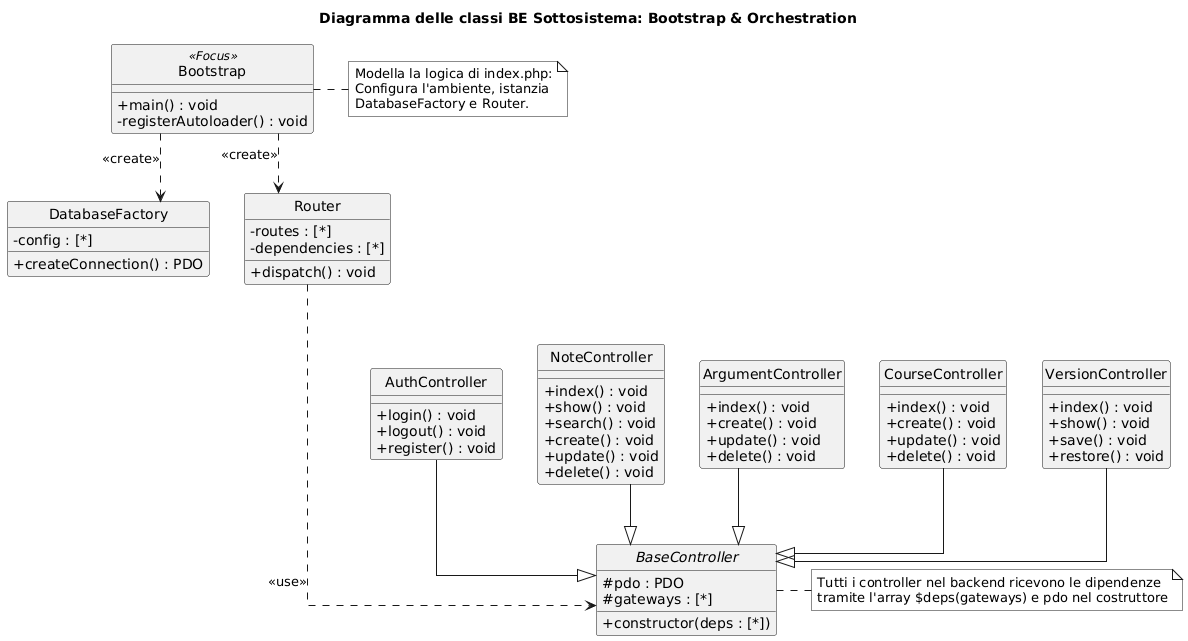
\includegraphics[width=1\textwidth]{DiagrammiClassi/DC_BE_EntryPoint.png}
    \caption{Diagramma delle classi BE Sottosistema: Bootstrap \& Orchestration}
    \label{fig:DC_BE_EntryPoint}
\end{figure}

\subsection{Diagramma delle classi BE Sottosistema: Persistence \& Security}

\noindent Il diagramma del sottosistema di persistenza e sicurezza formalizza l'architettura di accesso allo strato dei dati, strutturata mediante l'integrazione dei pattern \textit{Table Data Gateway} e \textit{Protection Proxy}. Il cuore strutturale è rappresentato dalla gerarchia che discende dalla classe astratta \texttt{AbstractGateway}, la quale centralizza il riferimento protetto all'oggetto \texttt{PDO} e fornisce i metodi necessari per la composizione sicura delle query SQL tramite \textit{Query Object}. In conformità ai requisiti di sicurezza (\textbf{RNF4}), l'accesso operativo ai dati è mediato da una serie di classi \texttt{Proxy} (es. \texttt{NotesGatewayProxy}) che realizzano le interfacce del sottosistema. Tali componenti permettono di intercettare ogni chiamata e verificare i privilegi dell'utente in sessione prima di delegare l'esecuzione effettiva, garantendo così che operazioni sensibili come la creazione o l'eliminazione siano riservate ai soli ruoli autorizzati. Il modulo \texttt{CascadeService} agisce come coordinatore per le procedure di eliminazione complessa, orchestrando l'interazione tra gateway differenti.

\begin{figure}[H]
    \centering
    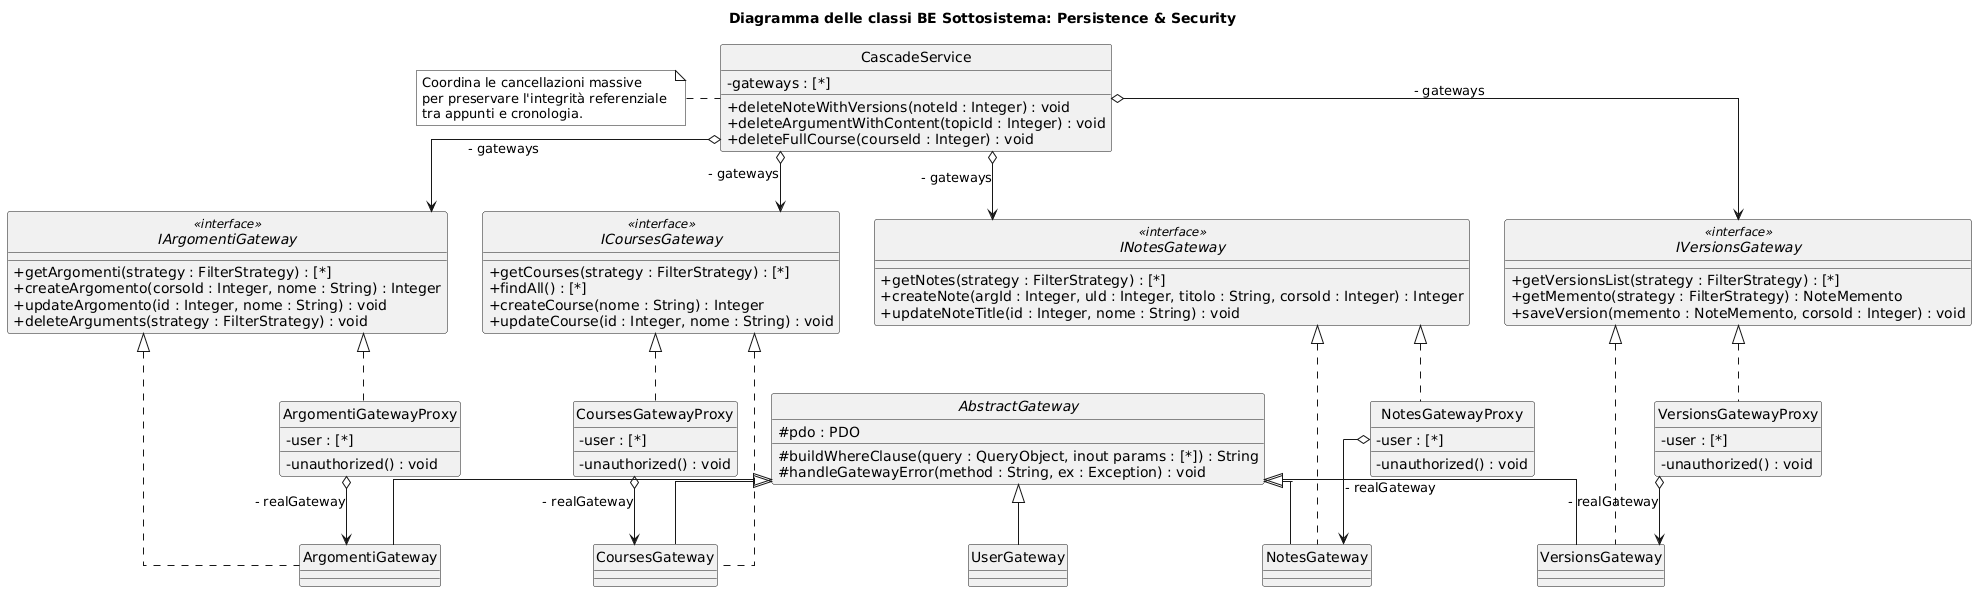
\includegraphics[width=1\textwidth]{DiagrammiClassi/DC_BE_TDG_Proxy.png}
    \caption{Diagramma delle classi BE Sottosistema: Persistence \& Security}
    \label{fig:DC_BE_TDG}
\end{figure}

\subsection{Diagramma delle classi BE Sottosistema: Strategy \& Query Object}

\noindent Il diagramma delle classi relativo al filtraggio delle risorse formalizza l'architettura utilizzata per la generazione dinamica dei criteri di ricerca, basata sull'integrazione dei pattern \textit{Strategy} e \textit{Query Object}. L'interfaccia \texttt{FilterStrategy} funge da astrazione centrale, definendo il contratto operativo \texttt{buildCriteria()} che permette di estendere il sistema con nuovi algoritmi di filtraggio (es. \texttt{SearchFilter} o \texttt{CourseFilter}) senza modificare i client esistenti, rispettando il principio \textit{Open/Closed}. Il disaccoppiamento tra la logica di dominio e la sintassi SQL è garantito dalla classe \texttt{QueryObject}. Tale struttura permette alle strategie concrete di popolare l'oggetto di query con requisiti logici (come l'operatore \texttt{LIKE} o \texttt{IN}), che verranno successivamente interpretati dall'infrastruttura di persistenza per produrre \textit{prepared statements} sicuri, assicurando così l'integrità del sistema contro attacchi di \textit{SQL Injection}.

\begin{figure}[H]
    \centering
    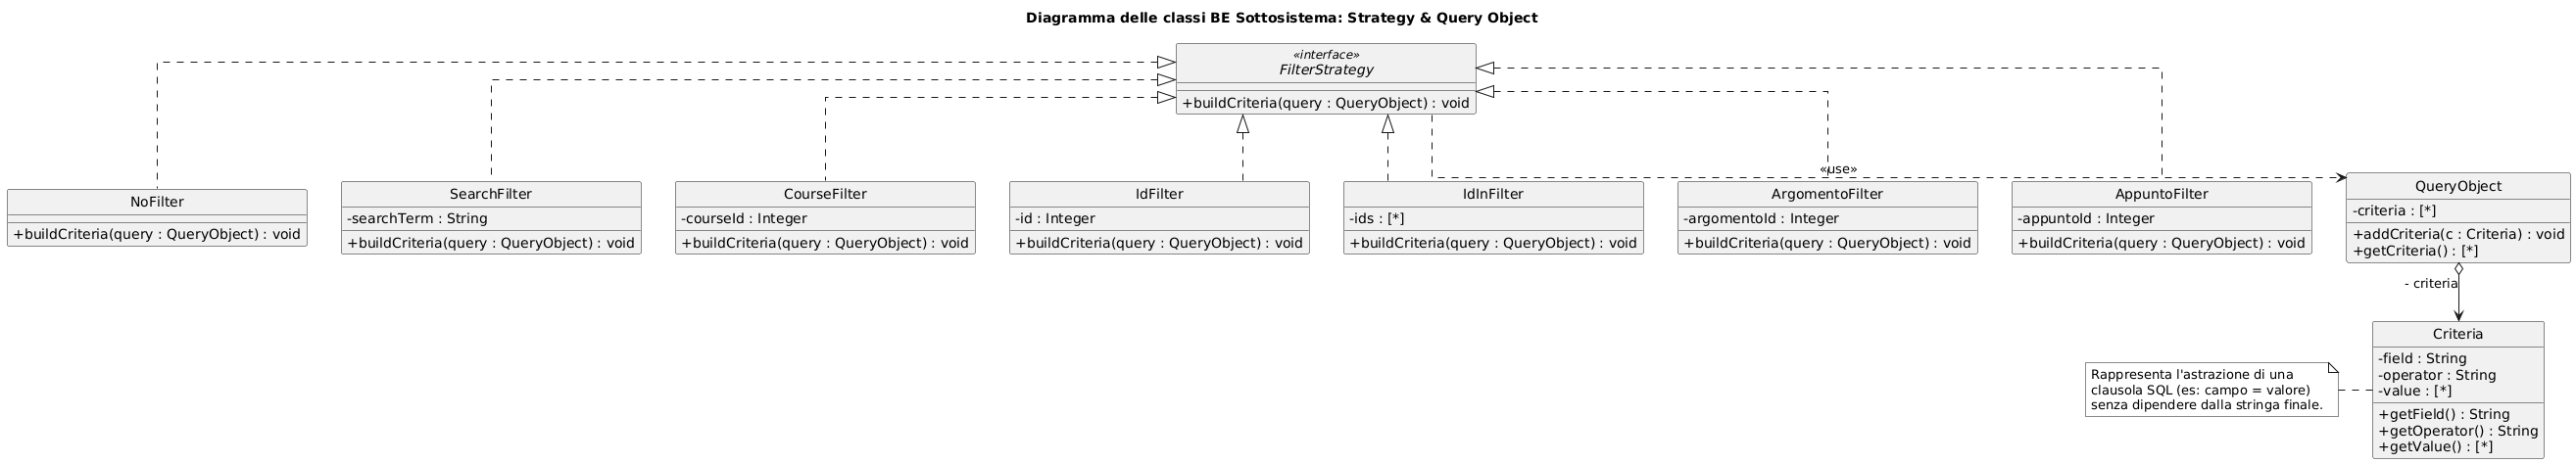
\includegraphics[width=1\textwidth]{DiagrammiClassi/DC_BE_Strategy.png}
    \caption{Diagramma delle classi BE Sottosistema: Strategy \& Query Object}
    \label{fig:DC_BE_Strategy}
\end{figure}

\subsection{Diagramma delle classi BE Sottosistema: Gestione Stato e Cronologia}

Il diagramma delle classi relativo alla persistenza e al ripristino degli appunti formalizza l'applicazione del pattern \textit{Memento}. La classe \texttt{Note} assume il ruolo di \textit{Originator}, detenendo lo stato interno dell'appunto e fornendo i metodi \texttt{saveToMemento()} e \texttt{restoreFromMemento()} per la generazione e il ripristino dei checkpoint. Il legame tra l'originatore e il componente \texttt{NoteMemento} è modellato tramite una \textit{Usage Dependency}, a indicare che la responsabilità dell'istanziazione dello stato spetta esclusivamente alla classe \texttt{Note}. \texttt{NoteMemento} definisce i propri attributi con visibilità privata e li mette a disposizione tramite il metodo \texttt{getState()}, assicurando che lo stato sia accessibile solo per fini di persistenza o ripristino autorizzato. \texttt{VersionsGateway} funge da \textit{Caretaker}, coordinando la custodia e il recupero dei memento dal database.


\begin{figure}[H]
    \centering
    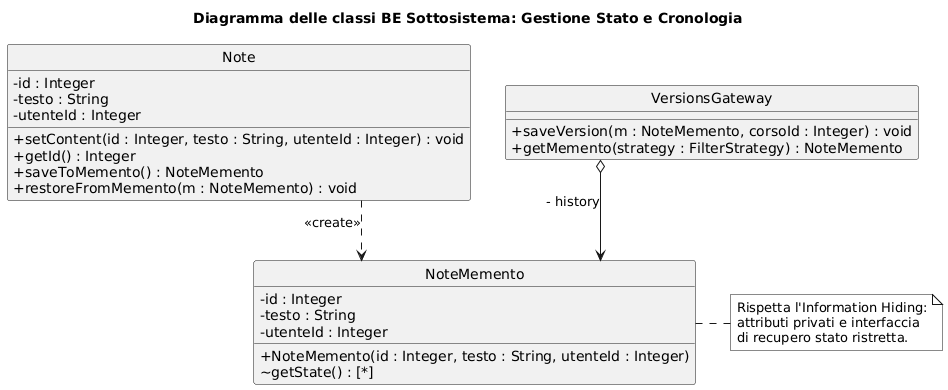
\includegraphics[width=1\textwidth]{DiagrammiClassi/DC_BE_Memento.png}
    \caption{Diagramma delle classi BE Sottosistema: Gestione Stato e Cronologia}
    \label{fig:DC_BE_Memento}
\end{figure}

\section{Diagrammi di Sequenza}

\noindent I seguenti diagrammi mostrano l'interazione temporale tra gli elementi dell'applicativo descrivendo alcuni casi d'uso e mettendo in luce l'uso di alcuni pattern.

\subsection{Diagramma di sequenza: RF6 (Creazione Appunto)}
Il diagramma di sequenza relativo alla creazione di un nuovo appunto formalizza l'integrazione del pattern \textit{Protection Proxy}. Il \texttt{NoteController}, operando come client dell'interfaccia \texttt{INotesGateway}, interagisce in modo trasparente con il \texttt{NotesGatewayProxy} senza conoscere la natura reale dell'oggetto di persistenza. Il cuore del meccanismo di sicurezza risiede nella logica del proxy, il quale intercetta l'invocazione del metodo \texttt{createNote()} e verifica che l'utente in sessione possieda il ruolo di ``studente''. Solo in caso di esito positivo del controllo autoritativo, il proxy delega l'operazione al \texttt{NotesGateway} reale di creazione dell'appunto.

\begin{figure}[H]
    \centering
    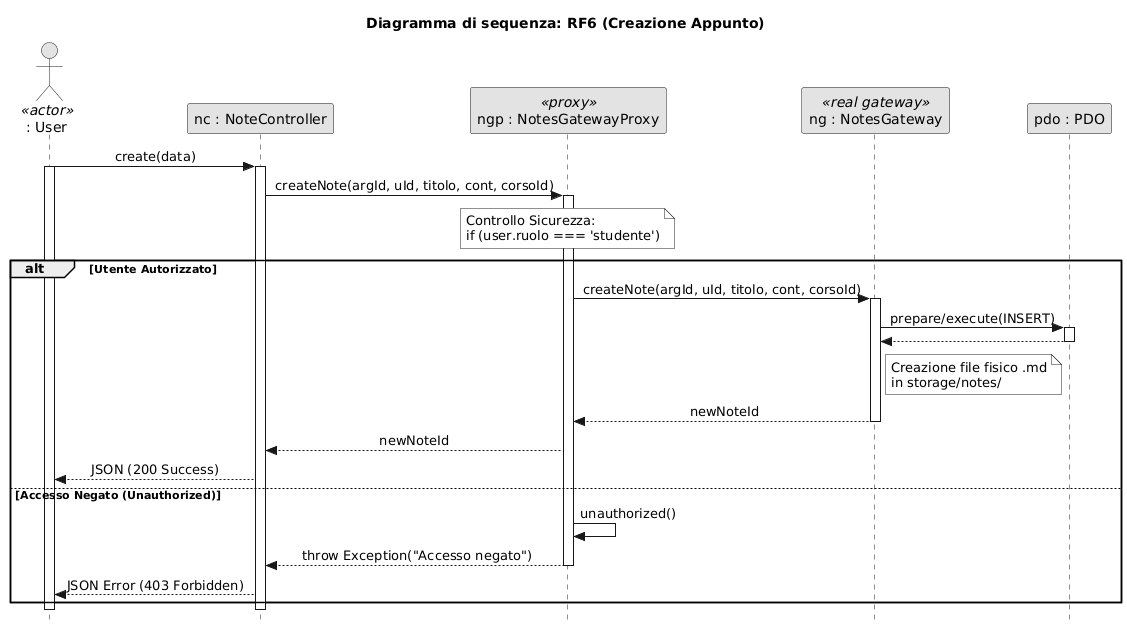
\includegraphics[width=1\textwidth]{DiagrammiSequenza/DS_RF6.png}
    \caption{Diagramma di sequenza: RF6 (Creazione Appunto)}
    \label{fig:DS_RF6}
\end{figure}


\subsection{Diagramma di sequenza: RF8 (parte Salvataggio Nuova Versione)}

Il diagramma di sequenza illustra la procedura di creazione di un checkpoint per un appunto applicando il pattern \textit{Memento}. Il processo è coordinato dal \texttt{VersionController}, il quale, dopo aver aperto una transazione tramite l'astrazione \texttt{PDO}, aggiorna l'oggetto \texttt{Note} (\textit{Originator}) e ne richiede la cattura dello stato tramite il metodo \texttt{saveToMemento()}. Quest'ultimo istanza un oggetto \texttt{NoteMemento} che incapsula le informazioni correnti in modo immutabile. Il \texttt{VersionsGateway} agisce come \textit{Caretaker}, ricevendo il memento e accedendo alla sua interfaccia ``stretta'' tramite il metodo \texttt{getState()} per persistere i dati sul database.

\begin{figure}[H]
    \centering
    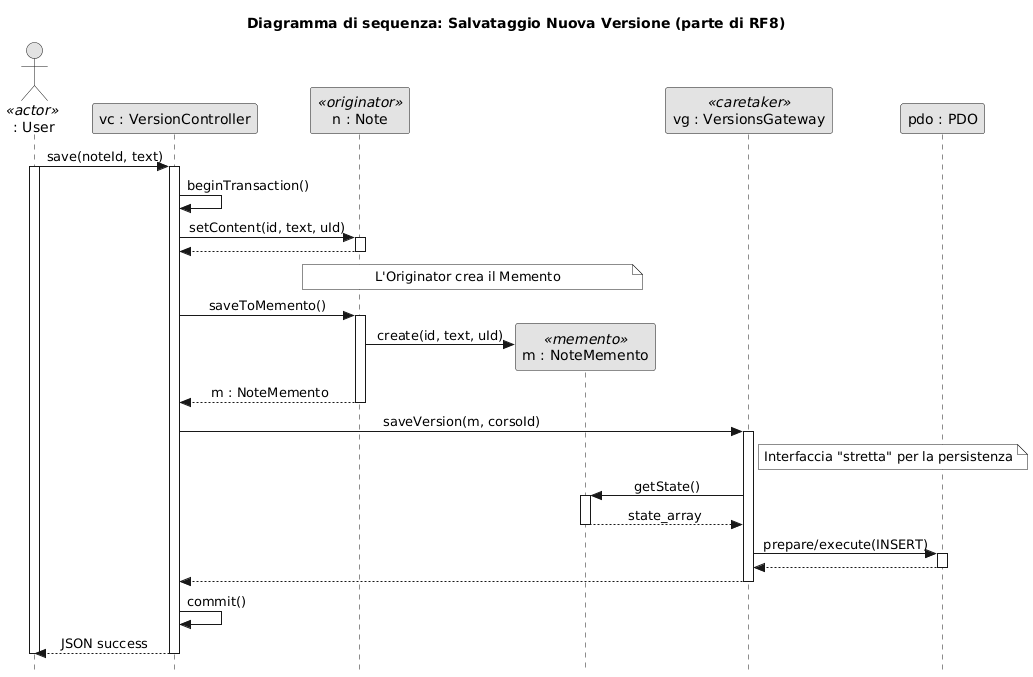
\includegraphics[width=1\textwidth]{DiagrammiSequenza/DS_RF8.png}
    \caption{Diagramma di sequenza: RF8 (parte Salvataggio Nuova Versione)}
    \label{fig:DS_RF8}
\end{figure}

\subsection{Diagramma di sequenza: RF9 (Ricerca Appunti)}

\noindent Il diagramma di sequenza per la ricerca (RF9) illustra l'applicazione del pattern \textbf{Strategy}, garantendo il \textbf{disaccoppiamento} tra logica di controllo e accesso ai dati. Il \texttt{NoteController} istanzia la strategia concreta \texttt{SearchFilter} e la passa al \texttt{NotesGateway} tramite il metodo \texttt{getNotes()}. Il gateway delega alla strategia il popolamento del \textbf{QueryObject} mediante \texttt{buildCriteria()}, applicando l'operatore \texttt{LIKE} sul titolo. Infine, il metodo \texttt{buildWhereClause} trasforma i criteri in un \textbf{prepared statement} SQL sicuro contro la \textbf{SQL Injection}. Questa architettura rispetta il principio \textbf{Open/Closed}, permettendo di aggiungere nuovi filtri senza modificare la struttura del gateway.

\begin{figure}[H]
    \centering
    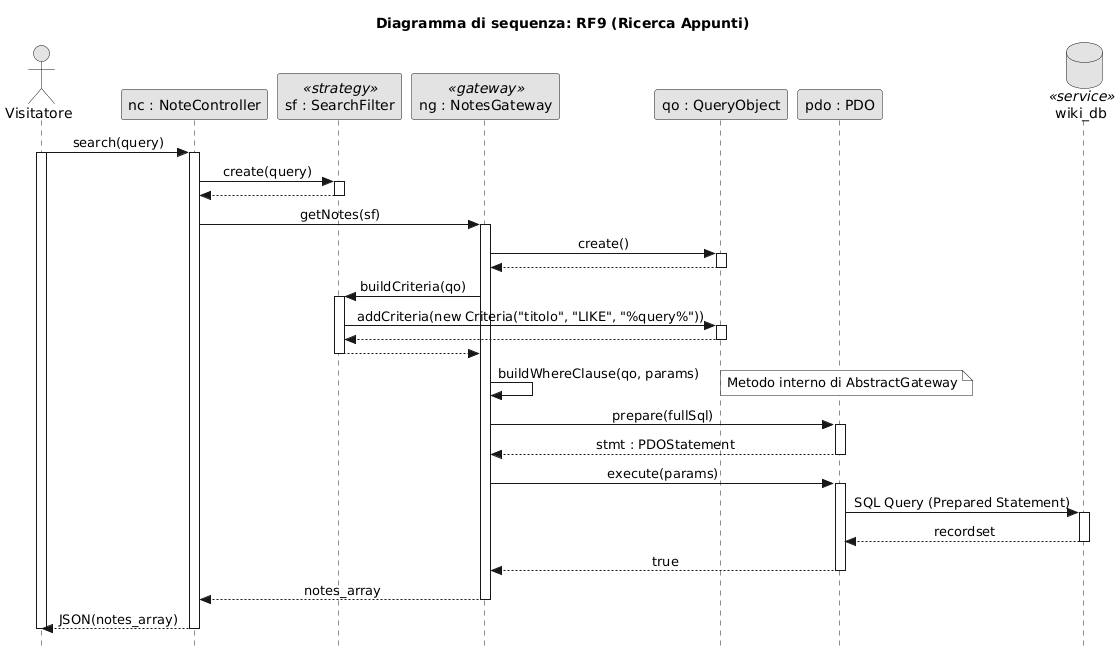
\includegraphics[width=1\textwidth]{DiagrammiSequenza/DS_RF9.png}
    \caption{Diagramma di sequenza: RF9 (Ricerca Appunti)}
    \label{fig:DS_RF9}
\end{figure}

\section{Diagrammi di Attività}

\noindent I diagrammi delle attività descrivono il flusso di controllo e le informazioni dei processi, supportando la modellazione di comportamenti paralleli. Nella progettazione software, questi grafici illustrano algoritmi e operazioni attraverso nodi, archi e partizioni (\textit{swimlanes}) per suddividere le responsabilità tra i componenti.


\subsection{Diagramma delle Attività: Login (RF2)}

\noindent Il diagramma delle attività per il \textbf{login (RF2)} illustra la verifica dell'identità. Il flusso parte dal \texttt{AppPresenter} (validazione sintattica) e passa al \texttt{AppModel}. Nel backend, l'\texttt{AuthController} coordina lo \texttt{UserGateway}, che applica la \textbf{Strategy} \texttt{EmailFilter} per il recupero dei dati. In linea con i requisiti di \textbf{sicurezza (RNF4)}, il sistema confronta l'\textbf{hash sha256} della password fornita con quello memorizzato. Eventuali errori sono gestiti da nodi di decisione che restituiscono uno stato \textbf{HTTP 401 (Unauthorized)}, mentre il successo determina l'avvio della sessione e il reindirizzamento dell'utente.


\begin{figure}[H]
    \centering
    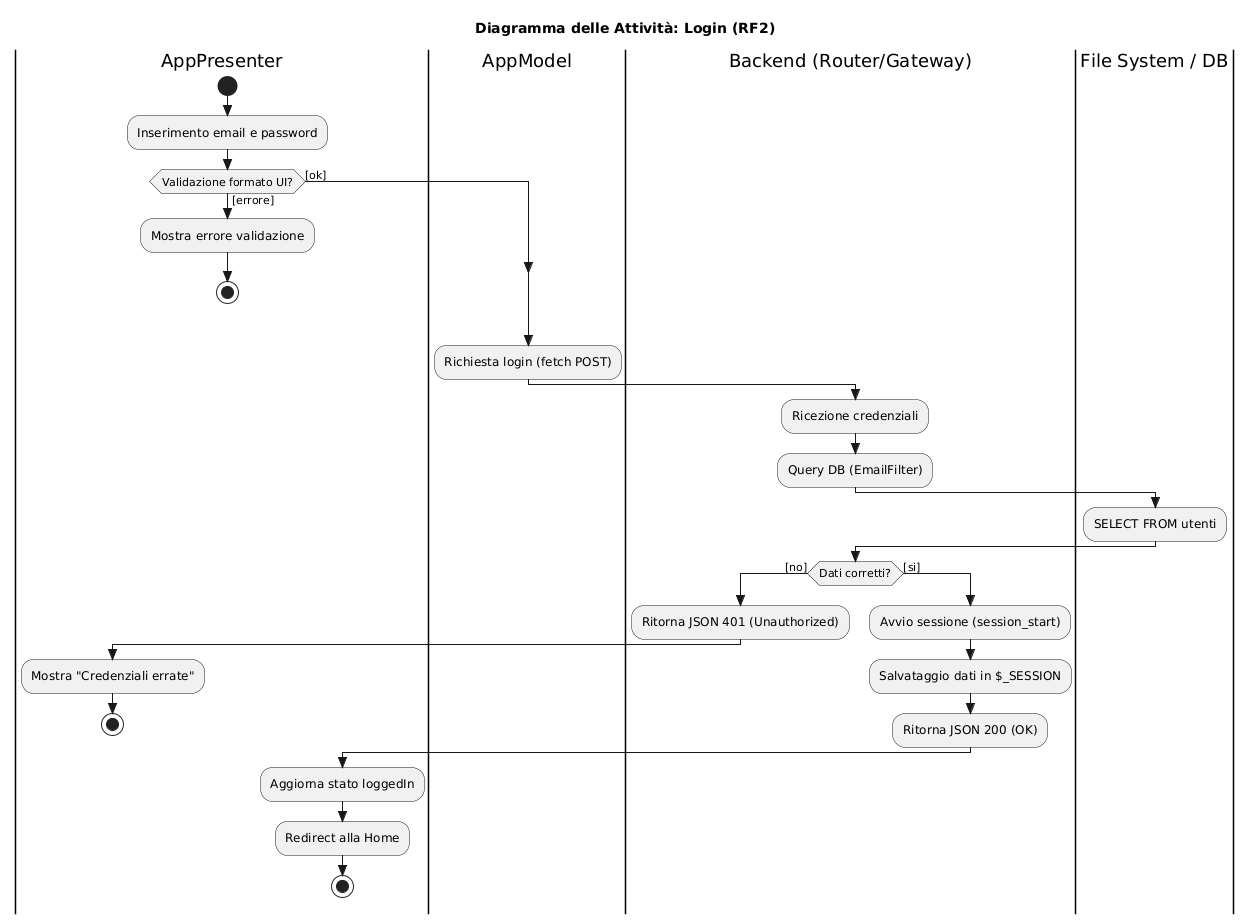
\includegraphics[width=1\textwidth]{DiagrammiAttivita/DA_RF2.png}
    \caption{Diagramma delle Attività: Login (RF2)}
    \label{fig:DA_RF2}
\end{figure}

\subsection{Diagramma delle Attività: Visualizza Appunto (RF5)}

\noindent Il seguente diagramma delle attività illustra il flusso di recupero di un appunto, caratterizzato dalla scomposizione della risorsa tra database relazionale e \textit{file system}. Il processo è innescato dal \texttt{AppPresenter} e mediato dal \texttt{AppModel} tramite una richiesta asincrona allo strato di \textit{backend}. Il \texttt{NotesGateway} esegue una query SQL per estrarre i metadati e il percorso relativo del file; successivamente, una struttura di controllo verifica l'esistenza fisica del documento Markdown nel \textit{file system}. Il punto critico del processo risiede nell'``Integrazione Dati'', fase in cui il gateway aggrega il record del database con il contenuto testuale letto dal disco prima di veicolare la risposta JSON completa verso il \textit{frontend}, garantendo la tracciabilità del requisito RF5 e la gestione degli errori in caso di file mancante.

\begin{figure}[H]
    \centering
    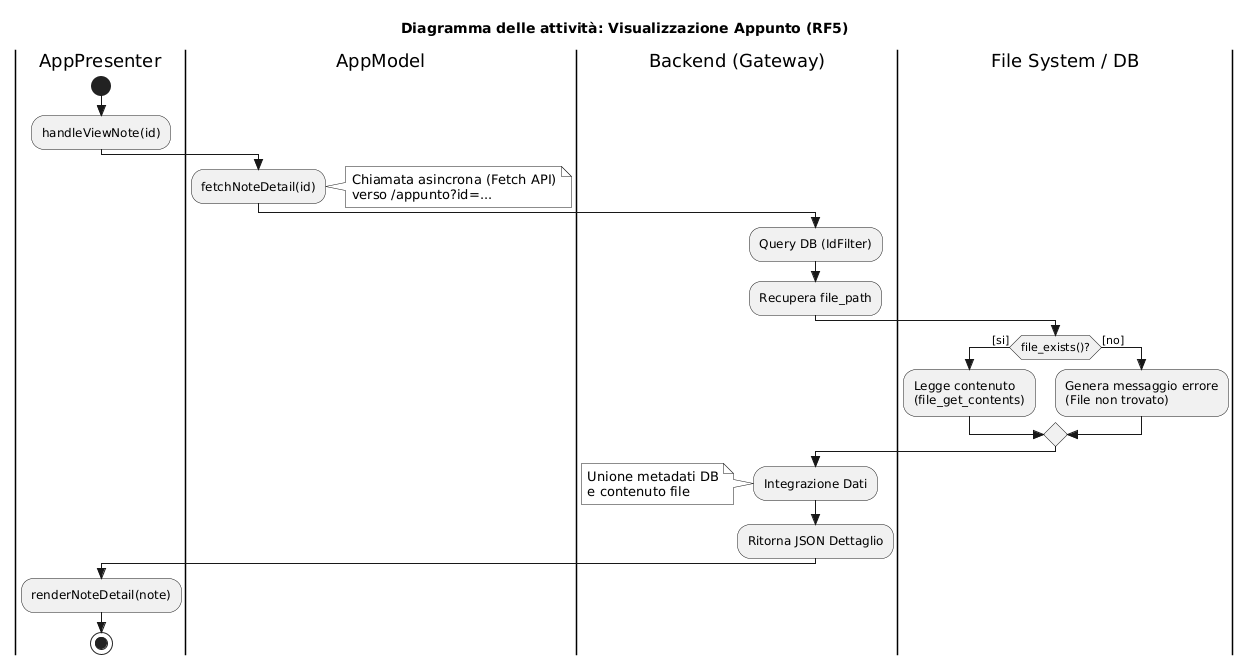
\includegraphics[width=1\textwidth]{DiagrammiAttivita/DA_RF5.png}
    \caption{Diagramma delle Attività: Visualizza Appunto (RF5)}
    \label{fig:DA_RF5}
\end{figure}


\section{Progettazione dei Dati}

\noindent Il sistema adotta un approccio di persistenza ibrido per ottimizzare la gestione di contenuti testuali variabili. Il database relazionale MySQL è incaricato della gestione della struttura logica. Il contenuto effettivo degli appunti e delle loro versioni non viene salvato nelle tabelle, ma archiviato direttamente nel file system del server. All'interno del database, i campi \texttt{file\_path} fungono da puntatori verso i file Markdown fisici, permettendo di unire la velocità di accesso al disco per file voluminosi con la coerenza dei metadati garantita dallo strato \texttt{SQL}.

\begin{figure}[H]
    \centering
    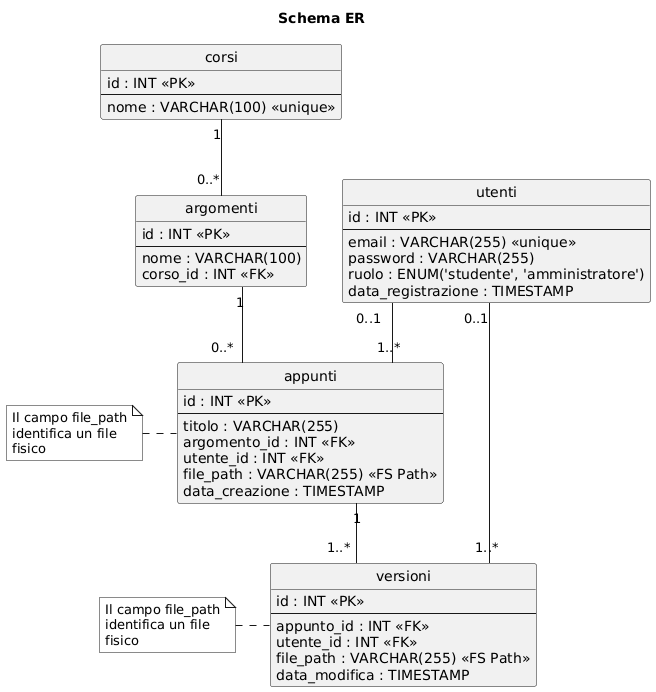
\includegraphics[width=0.8\textwidth]{AltriDiagrammi/DER.png}
    \caption{Schema Entity-Relationship}
    \label{fig:DER}
\end{figure}

\subsection{Organizzazione del File System}

\noindent I file sono organizzati in una struttura a directory che riflette la gerarchia logica del catalogo, facilitando la manutenzione e scalabilità del sistema. La radice del repository è la cartella \texttt{notes} (sotto \texttt{backend/storage/}), strutturata come segue:

\begin{center}
    \begin{minipage}{0.85\textwidth}
        \dirtree{%
        .1 notes/.
        .2 [ID\_Corso]/.
        .3 [ID\_Appunto].md \DTcomment{Versione attuale}.
        .3 versions/.
        .4 [ID\_Appunto]/.
        .5 v1.md \DTcomment{Versioni numerate progressivamente}.
        .5 v2.md.
        }
    \end{minipage}
\end{center}

\noindent L'utilizzo degli ID numerici come nomi di directory e file offre molteplici vantaggi tecnici:
\begin{enumerate}
    \item \textbf{Disaccoppiamento}: Il File System è indipendente dai titoli dei corsi o degli appunti, che possono essere rinominati nel database senza richiedere modifiche ai file.
    \item \textbf{Performance}: La segmentazione in sottodirectory previene il degrado delle prestazioni tipico dei file system con un numero eccessivo di file in un'unica cartella (flat directory).
    \item \textbf{Integrità}: La separazione netta tra la cartella dei contenuti "vivi" e la directory \texttt{versions/} riduce il rischio di sovrascritture accidentali durante le operazioni di manutenzione.
\end{enumerate}

\section{Specifica REST API}

\noindent La comunicazione tra il frontend (\textit{JavaScript}) e il backend (\textit{PHP}) del sistema Wiki Collaborativo avviene attraverso un’architettura di tipo \textbf{RESTful} (Representational State Transfer). Questa scelta garantisce un netto disaccoppiamento tra l'interfaccia utente e la logica di business, permettendo ai due componenti di evolvere indipendentemente e rendendo il sistema facilmente manutenibile e scalabile. Di seguito elenco i principi fondamentali del paradigma \textbf{REST}:

\begin{itemize}
    \item \textbf{Risorse e URI}: Ogni entità del dominio, come \textit{corsi}, \textit{argomenti} e \textit{appunti}, è trattata come una risorsa identificata univocamente da un \textbf{URI} (Uniform Resource Identifier) descrittivo e intuitivo, seguendo una struttura gerarchica coerente.
    
    \item \textbf{Protocollo Stateless}: Ogni richiesta inviata dal client al server è autocontenuta e include tutte le informazioni necessarie per l'elaborazione; al server non è richiesto di memorizzare lo stato del contesto dell'utente tra una chiamata e l'altra, favorendo la scalabilità del sistema.
    
    \item \textbf{Interfaccia Uniforme e CRUD}: Le interazioni avvengono tramite l'uso esplicito dei verbi standard \textbf{HTTP}, che mappano direttamente le operazioni \textbf{CRUD} \textit{(Create, Read, Update, Delete)} sulle risorse: \texttt{GET} per il recupero \textit{(Read)}, \texttt{POST} per la creazione \textit{(Create)}, \texttt{PUT} per l'aggiornamento \textit{(Update)} e \texttt{DELETE} per la rimozione \textit{(Delete)}.
    
    \item \textbf{Formato JSON}: Tutte le risposte prodotte dal backend sono strutturate in formato \textbf{JSON} (JavaScript Object Notation), garantendo un interscambio di dati leggero, facile da leggere per gli umani e semplice da interpretare per le macchine.
\end{itemize}

\noindent Questa interfaccia definisce il contratto formale tra client e server, basato sulla netta \textbf{Separation of Concerns}. Tale approccio assicura che il frontend possa essere teoricamente sostituito con tecnologie alternative (come applicazioni mobile o desktop) senza dover modificare la logica di persistenza e di business implementata nel backend.

\subsection{Endpoint}
Di seguito vengono dettagliati i principali endpoint.

\subsubsection{1. Registrazione utente (RF1)}
\begin{itemize}
    \item \textbf{URL:} \texttt{/register}
    \item \textbf{Metodo:} \texttt{POST}    
    \item \textbf{Parametri Query:} 
        \begin{itemize}
            \item \texttt{email} (obbligatorio).
            \item \texttt{password} (obbligatorio).
        \end{itemize}
    \item \textbf{Descrizione:} Riceve le credenziali dal frontend e crea un nuovo utente.
\end{itemize}
Esempio risposta di Successo (JSON):
\begin{verbatim}
{"status":"success","id":4}
\end{verbatim}

\subsubsection{2. Login (RF2)}
\begin{itemize}
    \item \textbf{URL:} \texttt{/login}
    \item \textbf{Metodo:} \texttt{POST}
    \item \textbf{Parametri Query:} 
        \begin{itemize}
            \item \texttt{email} (obbligatorio).
            \item \texttt{password} (obbligatorio).
        \end{itemize}
    \item \textbf{Descrizione:} Verifica la corrispondenza tra email e password hashata per avviare la sessione.
\end{itemize}
Esempio risposta di Successo (JSON):
\begin{verbatim}
{
    "status": "success",
    "user": {
        "id": 3,
        "email": "nico@studenti.unipr.it",
        "ruolo": "studente",
        "data_registrazione": "2026-01-31 18:18:59"
    }
}
\end{verbatim}

\subsubsection{3. Logout (RF2)}
\begin{itemize}
    \item \textbf{URL:} \texttt{/logout}
    \item \textbf{Metodo:} \texttt{POST}
    \item \textbf{Descrizione:} Invalida la sessione lato server e pulisce lo stato lato client.
\end{itemize}

\subsubsection{4. Visualizzazione Corsi (RF3)}
\begin{itemize}
    \item \textbf{URL:} \texttt{/corsi}
    \item \textbf{Metodo:} \texttt{GET}
    \item \textbf{Descrizione:} Restituisce l'array di tutti i corsi presenti nel database.
\end{itemize}
Esempio risposta di Successo (JSON):
\begin{verbatim}
[
  { "id": 1, "nome": "Informatica" },
  { "id": 2, "nome": "Matematica" }
]
\end{verbatim}

\subsubsection{5. Visualizzazione argomenti di un corso (RF4)}
\begin{itemize}
    \item \textbf{URL:} \texttt{/argomenti}
    \item \textbf{Metodo:} \texttt{GET}
    \item \textbf{Parametri Query:} 
        \begin{itemize}
            \item \texttt{corso\_id} (obbligatorio): Identificativo univoco del corso di riferimento. È un parametro obbligatorio affinché la richiesta vada a buon fine.
        \end{itemize}
    \item \textbf{Descrizione:} Permette di recuperare l'elenco di tutti gli argomenti associati a un determinato corso selezionato dall'utente.
\end{itemize}
Esempio risposta di Successo (JSON):
\begin{verbatim}
[
    {
        "id": 4,
        "nome": "Meccanica",
        "corso_id": 3
    },
    {
        "id": 5,
        "nome": "Termodinamica",
        "corso_id": 3
    }
]
\end{verbatim}


\subsubsection{6. Recupero Appunti per Argomento (RF4,RF5)}
\begin{itemize}
    \item \textbf{URL:} \texttt{/appunti}
    \item \textbf{Metodo:} \texttt{GET}
    \item \textbf{Parametri Query:} 
        \begin{itemize}
            \item \texttt{argomento\_id} (obbligatorio): Identificativo univoco dell'argomento scelto.
        \end{itemize}
    \item \textbf{Descrizione:} Questo endpoint permette di ottenere la lista di tutti gli appunti associati a un determinato argomento. Risponde alla necessità dell'utente di navigare all'interno della gerarchia Corso → Argomento per giungere alla risorsa finale.
\end{itemize}
Esempio risposta di Successo (JSON):
\begin{verbatim}
[
    {
        "id": 4,
        "titolo": "Meccanica Classica",
        "argomento_id": 4,
        "utente_id": 1,
        "file_path": "storage\/notes\/3\/meccanica_classica.md",
        "data_creazione": "2026-01-30 14:53:36"
    },
    {
        "id": 5,
        "titolo": "Meccanica Statistica",
        "argomento_id": 4,
        "utente_id": 1,
        "file_path": "storage\/notes\/3\/meccanica_statistica.md",
        "data_creazione": "2026-01-30 14:53:36"
    }
]
\end{verbatim}

\subsubsection{7. Visualizzazione degli appunti (RF5)}
\begin{itemize}
    \item \textbf{URL:} \texttt{/appunto}
    \item \textbf{Metodo:} \texttt{GET}
    \item \textbf{Parametri Query:} 
        \begin{itemize}
            \item \texttt{id} (obbligatorio): Identificativo univoco dell'appunto scelto.
        \end{itemize}
    \item \textbf{Descrizione:} Restituisce i metadati e il contenuto grezzo del file Markdown.
\end{itemize}
Esempio risposta di Successo (JSON):
\begin{verbatim}
{
    "id": 4,
    "titolo": "Meccanica Classica",
    "argomento_id": 4,
    "utente_id": 1,
    "file_path": "storage\/notes\/3\/meccanica_classica.md",
    "data_creazione": "2026-01-30 14:53:36",
    "contenuto": "# Meccanica classica\r\n\r\nLa **meccanica classica**[...]"
}
\end{verbatim}

\subsubsection{8. Ricerca (RF9)}
\begin{itemize}
    \item \textbf{URL:} \texttt{/cerca}
    \item \textbf{Metodo:} \texttt{GET}
    \item \textbf{Parametri Query:} 
        \begin{itemize}
            \item \texttt{q} (obbligatorio): Rappresenta il termine di ricerca inserito dall'utente. Il sistema backend processa la richiesta solo se la lunghezza di \texttt{q} è maggiore o uguale a 2 caratteri; in caso contrario, viene restituita una lista vuota per ottimizzare le prestazioni
        \end{itemize}
    \item \textbf{Descrizione:} Permette di filtrare la collezione globale degli appunti cercando una corrispondenza testuale all'interno dei titoli.
    \item \textbf{Risposta di Successo (JSON):}
\end{itemize}
\begin{verbatim}
[
    {
        "id": 1,
        "titolo": "Introduzione al Corso",
        "argomento_id": 1,
        "utente_id": 1,
        "file_path": "storage\/notes\/1\/introduzione_al_corso.md",
        "data_creazione": "2026-01-30 14:53:36"
    },
    {
        "id": 6,
        "titolo": "Introduzione alla Termodinamica",
        "argomento_id": 5,
        "utente_id": 1,
        "file_path": "storage\/notes\/3\/introduzione_alla_termodinamica.md",
        "data_creazione": "2026-01-30 14:53:36"
    }
]
\end{verbatim}

\subsubsection{9. Creazione appunti (RF6)}
\begin{itemize}
    \item \textbf{URL}: \texttt{/appunto/crea}
    \item \textbf{Metodo}: POST
    \item \textbf{Parametri Query:}
        \begin{itemize}
            \item \texttt{titolo} (obbligatorio)
            \item \texttt{argomento\_id} (obbligatorio)
            \item \texttt{utente\_id} (obbligatorio)
            \item \texttt{contenuto} (obbligatorio)
        \end{itemize}
    \item \textbf{Descrizione:} Permette a uno studente autenticato di creare un nuovo appunto. Il sistema salva i metadati nel database e crea fisicamente il file \texttt{.md} nello storage dedicato.
    \item \textbf{Risposta di Successo (JSON):}
\end{itemize}
\begin{verbatim}
{ "status": "success", "id": 15 }
\end{verbatim}

\subsubsection{10. Modifica appunti (RF7)}
\begin{itemize}
    \item \textbf{URL}: \texttt{/appunto/versione/salva}
    \item \textbf{Metodo}: POST
    \item \textbf{Body JSON:}
        \begin{itemize}
            \item \texttt{id} (obbligatorio): ID dell'appunto da modificare.
            \item \texttt{testo} (obbligatorio): Nuovo contenuto Markdown.
            \item \texttt{utente\_id} (obbligatorio): ID dello studente che effettua la modifica.
        \end{itemize}
    \item \textbf{Descrizione:} Sovrascrive il contenuto dell'appunto attuale e, contestualmente, applica il pattern \textit{Memento} archiviando lo stato precedente come una nuova versione nella cronologia.
    \item \textbf{Risposta di Successo (JSON):}
\end{itemize}
\begin{verbatim}
{ 
    "status": "success", 
    "message": "Cronologia aggiornata e modifiche salvate" 
}
\end{verbatim}

\subsubsection{11. Gestione corsi, argomenti e appunti (RF10)}
\begin{itemize}
    \item \textbf{URL} (Crea): \texttt{/corso/crea} e \texttt{/argomento/crea} (POST) 
    \item \textbf{URL} (Modifica): \texttt{/corso/modfica}, \texttt{/argomento/modfica} e \texttt{/appunto/modfica} (PUT)
    \item \textbf{URL} (Elimina): \texttt{/corso/elimina}, \texttt{/argomento/elimina} e \texttt{/appunto/elimina} (DELETE)
    \item \textbf{Parametri Body (Esempio Creazione):}
        \begin{itemize}
            \item \texttt{nome} (obbligatorio): Nome della nuova risorsa (corso/argomento).
            \item \texttt{id} (obbligatorio per modifiche ed eliminazioni).
        \end{itemize}
    \item \textbf{Descrizione:} Insieme di API protette dal \textit{Protection Proxy} riservate al ruolo \texttt{amministratore}. Le operazioni di eliminazione utilizzano il \texttt{CascadeService} per garantire la pulizia atomica di DB e File System.
    \item \textbf{Risposta di Successo (JSON):}
\end{itemize}
\begin{verbatim}
{ "status": "success" }
\end{verbatim}

\subsubsection{12. Cronologia delle versioni (RF8)}
\begin{itemize}
    \item \textbf{URL (Lista)}: \texttt{/appunto/storia?id=[ID\_APPUNTO]} (GET)
    \item \textbf{URL (Visualizza)}: \texttt{/appunto/versione/visualizza?versione\_id=[ID]} (GET)
    \item \textbf{URL (Ripristina)}: \texttt{/appunto/versione/ripristina} (POST)
    \item \textbf{Parametri Body (Ripristina):}
        \begin{itemize}
            \item \texttt{versione\_id} (obbligatorio): ID della versione memento da promuovere.
            \item \texttt{utente\_id} (obbligatorio): ID dell'utente che richiede il ripristino.
        \end{itemize}
    \item \textbf{Descrizione:} Gestione dello storico tramite pattern \textit{Memento}. Il ripristino recupera lo stato dal database e dal file system, archiviando lo stato corrente prima di sovrascriverlo.
    \item \textbf{Risposta di Successo (JSON - Ripristina):}
\end{itemize}
\begin{verbatim}
{ 
    "status": "success", 
    "message": "Versione ripristinata correttamente"
}
\end{verbatim} 
\chapter{Architettura}

\section{Design Pattern Model-View-Presenter (MVP)}
Il pattern MVP separa le responsabilità in tre componenti distinti: il \textbf{Model}, che incapsula la business logic e la persistenza; la \textbf{View}, che agisce come interfaccia passiva delegando ogni decisione al Presenter; e il \textbf{Presenter}, che funge da orchestratore. A differenza del pattern MVC, la View non osserva direttamente il Model, riducendo l'accoppiamento e facilitando il testing in isolamento.

\begin{figure}[H]
    \centering
    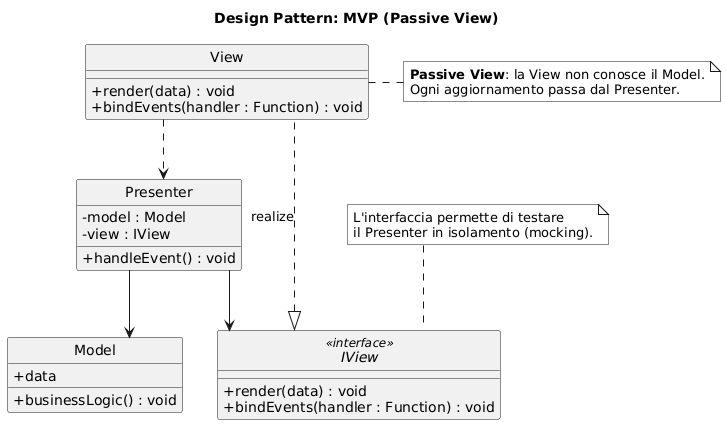
\includegraphics[width=0.8\textwidth]{DiagrammiDP/MVP.png}
    \caption{MVP}
    \label{fig:MVP}
\end{figure}

\subsection{Mapping nel codice}

\begin{itemize}
    \item \texttt{AppPresenter e AdminPresenter (Presenter)}: Fungono da mediatore; riceve gli input dalla View e coordina le richieste verso il Model, aggiornando l'interfaccia in base ai dati ricevuti.
    \item \texttt{AppModel (Model)}: Gestisce lo stato dei dati e l'interazione con le API REST del backend tramite richieste asincrone (\textit{Promises}).
    \item \texttt{BaseView, AppView, AuthView, AdminView, NoteView (View e IView)}: Rappresentano lo strato di visualizzazione (\textit{Passive View}); si occupano esclusivamente della manipolazione del DOM e del rendering dei corsi e degli appunti.
\end{itemize}

\section{Design Pattern Table Data Gateway}
Il pattern \textbf{Table Data Gateway} fornisce un oggetto che funge da gateway verso una specifica tabella del database. Esso contiene tutta la logica SQL \textit{(SELECT, INSERT, UPDATE, DELETE)} necessaria, isolando il resto dell'applicazione dai dettagli della persistenza. In genere restituisce un \textbf{RecordSet}, ovvero una struttura dati generica che mima la natura tabulare dei dati.

\begin{figure}[H]
    \centering
    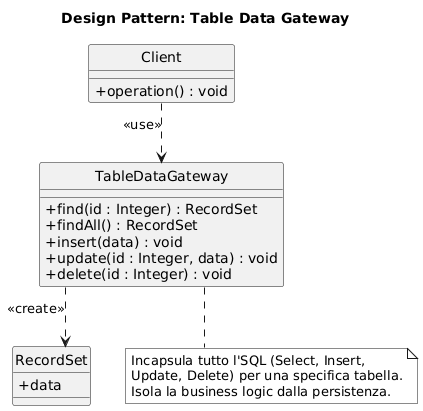
\includegraphics[width=0.6\textwidth]{DiagrammiDP/TDG.png}
    \caption{Table Data Gateway}
    \label{fig:TDG}
\end{figure}

\subsection{Mapping nel codice}

L'implementazione del sistema di persistenza segue una struttura gerarchica basata sul pattern \textbf{Table Data Gateway}, garantendo la separazione tra logica di business e accesso ai dati. Il mapping delle classi principali è articolato come segue:

\begin{itemize}
    \item \texttt{AbstractGateway} (Classe Base): Fornisce la logica comune a tutti i \textit{gateway}. Centralizza il metodo protetto \texttt{buildWhereClause()} il quale è fondamentale per trasformare i criteri astratti, definiti tramite il pattern \textit{Strategy}.
    
    \item \texttt{CoursesGateway}: Classe che gestisce la tabella \texttt{corsi}.
        
    \item \texttt{ArgomentiGateway}: Classe che gestisce la tabella \texttt{argomenti}.
    
    \item \texttt{NotesGateway}: Classe che gestisce la tabella \texttt{appunti}.
    
    \item \texttt{UserGateway}: Classe che gestisce la tabella \texttt{utenti}.
    
    \item \texttt{VersionsGateway}: Classe che gestisce la tabella \texttt{versioni}. Si occupa anche della persistenza degli stati storici degli appunti, interfacciandosi con il sistema di versionamento basato sul pattern \textit{Memento}.

\end{itemize}

\section{Design Pattern Strategy}
Il pattern \textbf{Strategy} è un pattern comportamentale utilizzato per definire una serie di algoritmi intercambiabili a runtime. Attraverso l'uso dell'aggregazione, il \textbf{Context} delega l'esecuzione del compito a un oggetto che realizza l'interfaccia \textbf{Strategy}.

\begin{figure}[H]
    \centering
    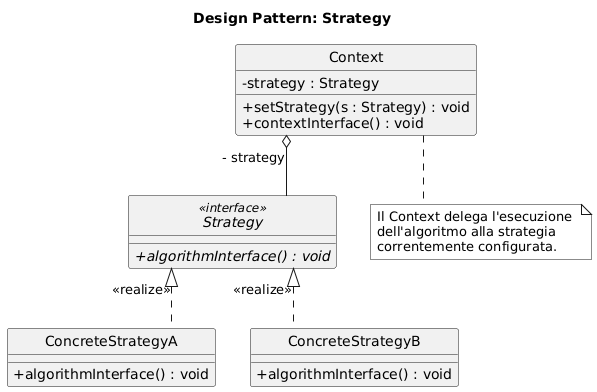
\includegraphics[width=0.8\textwidth]{DiagrammiDP/Strategy.png}
    \caption{Strategy}
    \label{fig:Strategy}
\end{figure}

\subsection{Mapping nel codice}

\begin{itemize}
    \item \texttt{FilterStrategy} (Interfaccia): \textit{Contratto} comune agli algoritmi di filtraggio. Definisce il metodo astratto \texttt{buildCriteria(QueryObject \$query)}, che obbliga ogni strategia concreta a popolare un oggetto di query con i criteri specifici del dominio.
    
    \item \texttt{CourseFilter}: Implementa il filtraggio degli argomenti in base all'identificativo di un corso specifico, in ottemperanza al requisito funzionale \textbf{RF4}.
    
    \item \texttt{ArgomentoFilter}: Filtro degli appunti in base all'identificativo di un argomento specifico.
    
    \item \texttt{SearchFilter}: Implementa la logica di ricerca testuale prevista dal requisito \textbf{RF9}. Istruisce il sistema a filtrare gli appunti il cui titolo corrisponde alla stringa inserita dall'utente tramite l'operatore SQL \texttt{LIKE} e l'utilizzo dei caratteri jolly \texttt{\%}.
    
    \item \texttt{IdFilter} e \texttt{EmailFilter}: Ulteriori specializzazioni del pattern utilizzate rispettivamente per recuperare il dettaglio di un singolo appunto (\textbf{RF5})o per estrarre le informazioni di un utente durante la procedura di \textit{login} tramite il campo \texttt{email} memorizzato nel database.

    \item \texttt{NoFilter}: Utilizzata per soddisfare il contratto \textbf{Strategy} quando non c'è bisogno di fare alcun filtro.

    \item \texttt{AppuntoFilter}: Permette di isolare le versioni appartenenti a uno specifico appunto, facilitando il recupero della cronologia (RF8).
    
    \item \texttt{IdInFilter}, \texttt{ArgomentiIdInFilter} e \texttt{AppuntoIdInFilter}: Strategie ottimizzate per la gestione di collezioni di identificativi tramite l'operatore \texttt{IN}. Sono componenti critici per il \texttt{CascadeService}, permettendo la rimozione atomica e sicura di record correlati in scenari di cancellazione massiva (RF10).

\end{itemize}

\section{Design Pattern Memento}

\noindent La gestione dello stato adotta il pattern \textbf{Memento}, garantendo l'incapsulamento dell'\texttt{Originator} tramite un'interfaccia ``stretta'' (\textit{narrow interface}). L'originatore crea i checkpoint mediante una \textit{Usage Dependency} (\guillemotleft\texttt{create}\guillemotright), mentre il \texttt{Caretaker} orchestra la cronologia dei dati. L'uso della molteplicità \texttt{[*]} per la proprietà \texttt{- history} assicura la gestione di una sequenza illimitata di stati, supportando operativamente l'\textit{undo} multi-livello.



\begin{figure}[H]
    \centering
    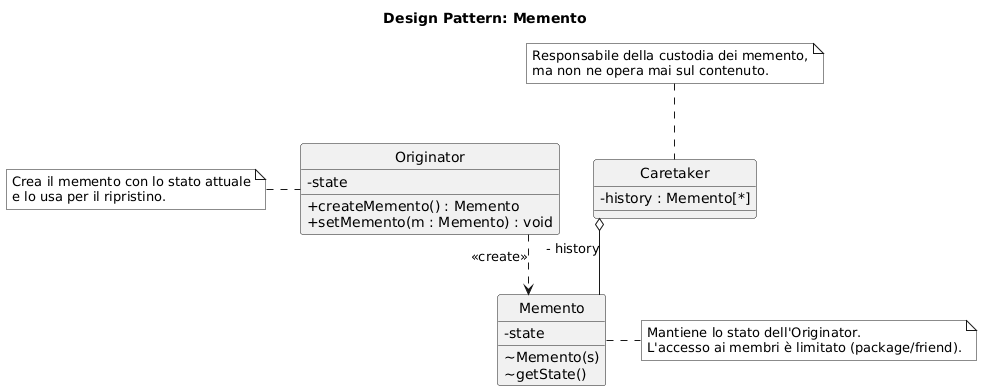
\includegraphics[width=1\textwidth]{DiagrammiDP/Memento.png}
    \caption{Memento}
    \label{fig:Memento}
\end{figure}


\subsection{Mapping nel codice}

\noindent L'implementazione del pattern \textbf{Memento} è distribuita tra le classi che gestiscono lo stato dell'appunto e lo strato di persistenza della cronologia:
\begin{itemize} 
    \item \texttt{Note}: Svolge il ruolo di \textit{Originator}. Detiene lo stato interno dell'appunto (testo, autore, ID) e implementa i metodi \texttt{saveToMemento()} per creare un'istantanea e \texttt{restoreFromMemento()} per il ripristino di uno stato precedente. 
    \item \texttt{NoteMemento}: Rappresenta l'oggetto \textit{Memento}. Incapsula i dati in modo immutabile e protegge l'incapsulamento fornendo lo stato tramite l'interfaccia stretta \texttt{getState()}, accessibile solo dall'Originator o dal Gateway di persistenza. 
    \item \texttt{VersionsGateway}: Agisce come \textit{Caretaker}. È l'unico componente responsabile della custodia fisica dei memento, gestendo la loro scrittura nel database (\texttt{saveVersion}) e il recupero dal file system. 
    \item \texttt{VersionController}: Coordina il flusso operativo, istruendo l'Originatore a generare il memento e delegando al Caretaker la sua conservazione all'interno di una transazione atomica. 
\end{itemize}

\section{Design Pattern Protection Proxy}

Il pattern Protection Proxy si configura come un'architettura di intermediazione in cui un oggetto $\texttt{Proxy}$ agisce da surrogato per un $\texttt{RealSubject}$, regolandone l'accesso in modo rigoroso. L'elemento cardine di tale struttura è l'astrazione definita dal $\texttt{Subject}$, che funge da contratto formale tra il sistema e il $\texttt{Client}$. Grazie a questo disaccoppiamento, il $\texttt{Client}$ interagisce esclusivamente con l'interfaccia astratta, ignorando se l'esecuzione avvenga tramite l'oggetto reale o il suo sostituto. Questa trasparenza operativa permette al sistema di evolvere e di integrare nuove logiche di sicurezza senza impattare minimamente sulle dipendenze esterne o sul codice chiamante.


\begin{figure}[H]
    \centering
    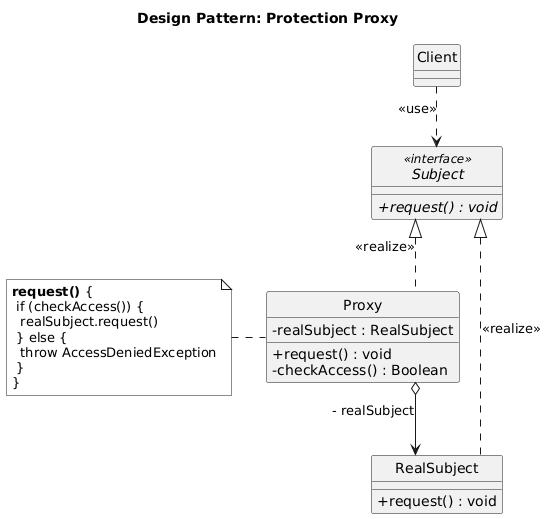
\includegraphics[width=0.8\textwidth]{DiagrammiDP/ProtectionProxy.png}
    \caption{Protection Proxy}
    \label{fig:ProtectionProxy}
\end{figure}


\subsection{Mapping nel codice}

\noindent La logica di sicurezza autoritativa è implementata tramite una serie di \textbf{Proxy} che filtrano l'accesso ai componenti di persistenza reale:
\begin{itemize} 
    \item \texttt{INotesGateway}, \texttt{IArgomentiGateway}, \texttt{IVersionsGateway}, \texttt{ICoursesGateway}: Definiscono l'interfaccia \textit{Subject}, che funge da contratto formale sia per il proxy che per il gateway reale, garantendo la trasparenza per il client (Controller). 
    \item \texttt{NotesGatewayProxy} e \texttt{VersionsGatewayProxy}: Implementano il ruolo di \textit{Proxy} per le risorse dinamiche. Intercettano le chiamate a metodi sensibili (come \texttt{createNote} o \texttt{saveVersion}), verificano il ruolo \texttt{studente} e negano l'accesso in caso di privilegi insufficienti.
    \item \texttt{NotesGateway}, \texttt{ArgomentiGateway}, \texttt{CoursesGateway} e \texttt{VersionsGateway}: Rappresentano i \textit{RealSubject}. Contengono la logica SQL (\texttt{PDO}) effettiva e la gestione del file system. Vengono invocati dai rispettivi proxy solo dopo il superamento con successo dei controlli autoritativi.
    \item \texttt{CoursesGatewayProxy} e \texttt{ArgomentiGatewayProxy}: Specializzazioni del proxy che proteggono la struttura del catalogo, riservando le operazioni di modifica ed eliminazione esclusivamente agli utenti con ruolo \texttt{amministratore}. 
\end{itemize}
 
\chapter{Piano di Test}

\section{Introduzione alla Validazione}
\noindent Il presente Piano di Test definisce le procedure necessarie per verificare che il sistema \textit{Wiki Collaborativo} sia conforme alle specifiche e soddisfi i bisogni reali degli utenti (\textit{Verifica \& Validazione}). La strategia adottata si basa sul \textbf{black-box testing}, in cui i casi di test sono derivati direttamente dai requisiti funzionali (RF) e non funzionali (RNF), testando il sistema tramite input selezionati per coprire sia scenari di successo che condizioni di errore.

\section{Casi di Test e Tracciabilità}
\noindent Ogni test case è progettato per garantire la \textbf{tracciabilità} verso il relativo requisito, assicurando che ogni funzionalità sia verificabile e correttamente implementata.

\begingroup
\renewcommand{\arraystretch}{1.5}
\small
% L'opzione [c] assicura il centraggio rispetto ai margini della pagina
\begin{longtable}[c]{|p{0.11\textwidth}|p{0.18\textwidth}|p{0.29\textwidth}|p{0.29\textwidth}|}
    
    % --- Intestazione iniziale (solo prima pagina) ---
    \hline
    \textbf{ID Test} & \textbf{Requisito} & \textbf{Input / Scenario} & \textbf{Risultato Atteso} \\ \hline
    \endfirsthead

    % --- Intestazione per le pagine successive ---
    \hline
    \multicolumn{4}{|c|}{{\footnotesize\itshape Continua dalla pagina precedente}} \\ \hline
    \textbf{ID Test} & \textbf{Requisito} & \textbf{Input / Scenario} & \textbf{Risultato Atteso} \\ \hline
    \endhead

    % --- Piè di pagina per le pagine intermedie ---
    \hline
    \multicolumn{4}{|r|}{{\footnotesize\itshape Continua nella prossima pagina}} \\ \hline
    \endfoot

    % --- Piè di pagina finale ---
    \hline
    \endlastfoot

    % --- Corpo della tabella (testo invariato) ---
    \texttt{T1} & RF1 & Inserimento di dati validi per un nuovo utente. & Status 200 (Success), nuovo utente generato correttamente. \\ \hline
    \texttt{T2} & RF1 & Registrazione con una email già presente nel database. & Status 409 (Conflict), messaggio "Email già registrata". \\ \hline
    \texttt{T3} & RF2 & Inserimento di password errata durante il login. & Status 401 (Unauthorized), accesso negato. \\ \hline
    \texttt{T4} & RF2 & Inserimento di password corretta durante il login. & Status 200 (Success), accesso autorizzato. \\ \hline
    \texttt{T5} & RF6 & Accesso alla pagina di un argomento come utente non autenticato (Visitatore). & Il pulsante "+ Crea Nuovo Appunto" non è presente nel DOM. \\ \hline
    \texttt{T6} & RF6 \& RNF4 & Invio manuale di una richiesta POST all'endpoint /appunto/crea senza una sessione valida. & Status 403 (Forbidden), intercettazione del \textit{Protection Proxy}. \\ \hline
    \texttt{T7} & RF10 \& RNF4 & Accesso con ruolo \texttt{studente} e tentativo di invio manuale di una richiesta DELETE all'endpoint \texttt{/corso/elimina}. & Status 403 (Forbidden), operazione negata dal Proxy. \\ \hline
    \texttt{T8} & RNF4 & \textbf{Ispezione persistenza}: Verifica del record utente nel DB dopo la registrazione. & Password memorizzate esclusivamente come hash \texttt{sha256}. \\ \hline
    \texttt{T9} & RF9 & Ricerca del titolo di un appunto con una stringa inferiore a 2 caratteri. & La ricerca non viene avviata dal frontend (ottimizzazione). \\ \hline
    \texttt{T10} & RF7 & Modifica di un appunto esistente da parte di uno studente autenticato. & Aggiornamento del file \texttt{.md} e creazione di un record in \texttt{versioni}. \\ \hline
    \texttt{T11} & RF10 \& RNF4 & Eliminazione di un argomento da parte di un utente con ruolo \texttt{amministratore}. & Status 200 (Success), pulizia tramite \textit{CascadeService}. \\ \hline
    \texttt{T12} & RF3 \& RF4 & Navigazione tra i corsi e argomenti. & Visualizzazione corretta della gerarchia nel frontend. \\ \hline
    \texttt{T13} & RF5  & Apertura di un appunto esistente. & Rendering HTML corretto da sorgente Markdown; metadati coerenti con il DB. \\ \hline
    \texttt{T14} & RF8  & Visualizzazione delle versioni. & Lista mostrata con timestamp e autore; anteprima disponibile nel modale. \\ \hline
    \texttt{T15} & RF8  & Ripristino di una versione. & Promozione della versione a corrente; ricaricamento dell'appunto aggiornato. \\ \hline
    \texttt{T16} & RF8  & Visualizzazione cronologia vuota. & Messaggio: "Nessuna versione precedente disponibile." \\ \hline
    \texttt{T17} & RF9  & Ricerca di un titolo esistente con stringa valida (es. "Meccanica"). & Restituzione dell'array JSON contenente i match corrispondenti. \\ \hline
    \texttt{T18} & RF2  & Esecuzione Logout. & Distruzione del token/sessione; reindirizzamento alla vista ospite. \\ \hline
    
    \caption{Tabella dei Casi di Test: Scenari di Validazione}
    \label{tab:test_plan}
\end{longtable}
\endgroup



\section{Considerazioni sulla Robustezza}
\noindent Il sistema è stato testato per gestire le anomalie tramite la generazione di eccezioni nello strato dei \textit{Gateway} e dei \textit{Proxy}. In particolare, l'uso di \textbf{prepared statements} SQL garantisce la robustezza contro attacchi di \textit{SQL Injection}.
 
\chapter{Manuale Tecnico}

\section{Introduzione}
Il sistema \textbf{Wiki UNIPR} è progettato per essere eseguito in un ambiente containerizzato tramite \textbf{Docker}. Questa architettura garantisce che il software funzioni in modo identico su qualsiasi macchina, isolando le dipendenze del Backend (PHP), del Database (MySQL) e del Frontend (Apache).

\section{Requisiti di Sistema}
Prima di procedere, assicurarsi che i seguenti strumenti siano installati e correttamente configurati:
\begin{itemize}
    \item \textbf{Docker Desktop} (Windows/macOS) o \textbf{Docker Engine} (Linux).
    \item \textbf{Docker Compose} (solitamente incluso nelle versioni recenti di Docker).
    \item Un terminale (Bash, PowerShell o WSL).
\end{itemize}

\section{Inizializzazione del Database}
Il database viene configurato automaticamente durante il primo avvio del container DB. 
\subsection{Logica di Popolamento}
Docker esegue gli script SQL presenti nella cartella \texttt{./services/database/configs/} seguendo l'ordine alfabetico dei nomi dei file. Per questo motivo, i file sono stati nominati con un prefisso numerico:

\begin{enumerate}
    \item \textbf{\texttt{01\_init.sql}}: Contiene i comandi \texttt{DROP DATABASE IF EXISTS} e \texttt{CREATE DATABASE} per garantire un ambiente pulito, seguiti dalla creazione delle tabelle con i relativi vincoli di integrità.
    \item \textbf{\texttt{02\_dump.sql}}: Contiene gli \texttt{INSERT} iniziali per popolare la tabella \texttt{corsi}, gli argomenti di test e gli utenti predefiniti.
\end{enumerate}

\section{Script di Automazione}
Per semplificare la gestione dell'ambiente, sono stati predisposti tre script \texttt{.sh} nella root del progetto.

\subsection{Avvio del Progetto (\texttt{run\_project.sh})}
Utilizzare questo script per avviare l'intero stack. Lo script richiede all'utente se desidera effettuare un reset dei volumi per ricaricare il database da zero.
\begin{verbatim}
./run_project.sh
\end{verbatim}

\subsection{Arresto del Progetto (\texttt{stop\_project.sh})}
Ferma i container in esecuzione senza eliminare i dati salvati nel database.
\begin{verbatim}
./stop_project.sh
\end{verbatim}

\subsection{Reset Totale (\texttt{reset\_all.sh})}
Elimina container, volumi e immagini, ricostruendo l'ambiente da uno stato pulito. Utile in caso di modifiche strutturali al file \texttt{init.sql}.
\begin{verbatim}
./reset_all.sh
\end{verbatim}

\section{Procedura di Installazione Standard}
\begin{enumerate}
    \item Clonare il repository o estrarre i file del progetto.
    \item Aprire il terminale nella cartella principale.
    \item Fornire i permessi di esecuzione agli script:
    \begin{verbatim}
chmod +x *.sh
    \end{verbatim}
    \item Eseguire lo script di avvio:
    \begin{verbatim}
./run_project.sh
    \end{verbatim}
    \item Almeno al primo avvio alla domanda su reset rispondere S
    \begin{verbatim}
Vuoi resettare il database e lo storage? (Perderai i dati correnti) [S/N]
    \end{verbatim}
    \item Attendere circa 10-15 secondi per consentire a MySQL di completare l'inizializzazione.
    \item Accedere all'app tramite browser all'indirizzo:
        \begin{verbatim}
http://localhost:8080
        \end{verbatim}
\end{enumerate}

\section{Credenziali di Test}
Per verificare le funzionalità del sistema (Login, consultazione e permessi), sono stati predisposti i seguenti account nel file di dump:


\begin{table}[h!]
\centering
\caption{Credenziali di test pre-caricate nel sistema.}
\label{tab:credenziali}
\resizebox{\textwidth}{!}{% <-- Inizio ridimensionamento
\begin{tabular}{|l|l|l|l|}
\hline
\textbf{Tipo Utente} & \textbf{Email} & \textbf{Password} & \textbf{Ruolo} \\ \hline
Amministratore & \texttt{admin@unipr.it} & \texttt{Vector!} & \texttt{amministratore} \\ \hline
Studente & \texttt{studente\_test1@studenti.unipr.it} & \texttt{Prova1} & \texttt{studente} \\ \hline
Studente & \texttt{studente\_test2@studenti.unipr.it} & \texttt{Prova2} & \texttt{studente} \\ \hline
Studente & \texttt{studente\_test3@studenti.unipr.it} & \texttt{Prova3} & \texttt{studente} \\ \hline
\end{tabular}% <-- Fine ridimensionamento
}
\end{table}


\section{Risoluzione dei Problemi}
Se le tabelle non dovessero risultare presenti (\textit{Table not found}), eseguire il comando \texttt{./reset\_all.sh}. Questo forzerà Docker a cancellare il volume dati esistente e a rieseguire gli script di inizializzazione \texttt{01\_init.sql} e \texttt{02\_dump.sql}.

 

\end{document}
